\chapter{Analyse van Observatieprestaties}
\label{ch:analyse}

\section{Inleiding}

In de voorgaande hoofdstukken werden de ontwikkeling van de PoC applicatie, de methodologie voor het verzamelen 
van experimentele data, en het creëren van een grondwaarheidsdataset uitvoerig besproken. 
Dit hoofdstuk richt zich op de kern van het onderzoek: de geautomatiseerde analyse van de 
observatieprestaties van studenten aan de hand van de verzamelde eyetracking-opnames.

Het hoofddoel van de hier beschreven analyse is, om op basis van de videofeed en blikdata van de Tobii Pro Glasses 3, 
automatisch te bepalen (1) welke van de vooraf gedefinieerde kritische objecten door een student zijn waargenomen en (2) 
hoe lang de aandacht op elk van deze objecten gericht was. 
Om dit te realiseren, werd een analysepipeline ontworpen en geïmplementeerd, die de output van verschillende computervisiemodellen combineert.

De ontwikkelde analysepipeline, zoals conceptueel voorgesteld in Strategie 4 van Hoofdstuk~\ref{ch:oplossingsstrategieen}, 
transformeert de ruwe video- en blikdata, frame-per-frame tot een identificatie van bekeken, kritische objecten. 
Dit proces omvat drie hoofdfasen: (1) het segmenteren en tracken van alle potentiële objecten in beeld, 
(2) het filteren van deze segmenten op basis van objectgrootte en daadwerkelijke observatie door de student, en 
(3) het classificeren van de overgebleven objectsegmenten. 
Er werden drie verschillende benaderingen voor de classificatiestap geëvalueerd:
\begin{enumerate}
  \item \textbf{Vector-Index Classificatie:} Hierbij worden eerst image embeddings van de bekeken segmenten gegenereerd met DINOv2.
  Hierna worden deze embeddings vergeleken met voorbeelden van de kritische objecten binnen een\\ \texttt{Faiss (Facebook AI Similarity Search)} vector-index.
  \item \textbf{YOLOv11 Classificatie:} In deze benadering wordt een YOLOv11-model\\ getraind om de segmenten te classificeren.
  \item \textbf{YOLOv11 Object Detectie:} Deze aanpak verschilt van de vorige doordat het model niet enkel classificeert, 
  maar ook de locatie van de objecten in het frame bepaalt. 
  De objectdetector genereert bounding boxes, die vervolgens worden gecombineerd met de trackingresultaten van FastSAM om tot een definitieve classificatie te komen van elk bekeken object.
\end{enumerate}
Merk op dat het bij de eerste fase niet enkel over frame-per-frame segmentatie gaat, maar ook over het tracken van deze segmenten doorheen de video.
Deze aanpak maakt het mogelijk om na classificatie van de individuele segmenten, de resultaten te aggregeren over de volledige tracking-sessie van elk object. 

De ontwikkelde methoden werden beoordeeld aan de hand van de in Hoofdstuk~\ref{ch:grondwaarheid} gecreëerde grondwaarheid.

Figuur~\ref{fig:analyse-pipeline-visualisatie} illustreert de fasen van dit proces aan de hand van illustratieve beelden.

\begin{figure}[H]
    \centering
        \begin{subfigure}[b]{0.75\textwidth}
        \centering
        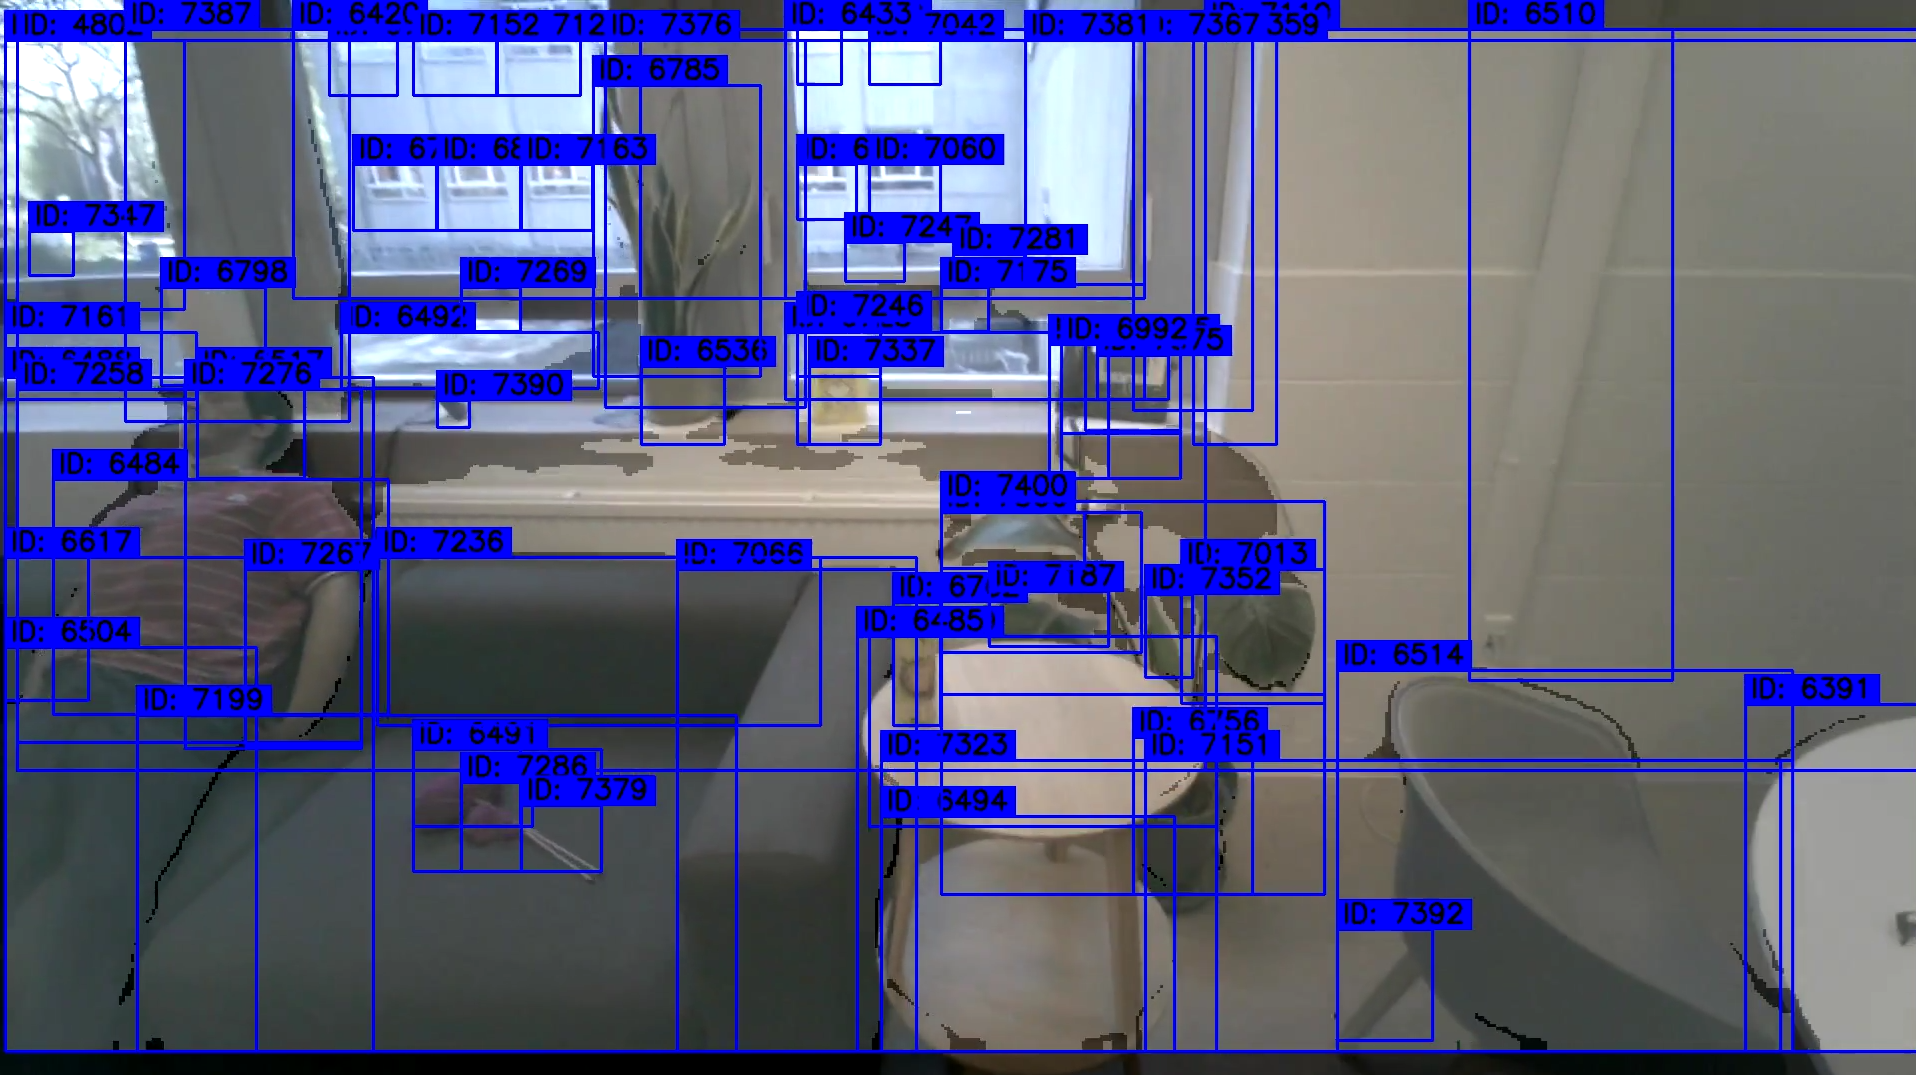
\includegraphics[width=1\textwidth]{everything-prompt.png}
        \caption{Everything-Segmentatie (FastSAM)}
        \label{fig:pipeline_stap_a}
    \end{subfigure}

    \vspace{0.5cm}

    \begin{subfigure}[b]{0.75\textwidth}
    \centering
    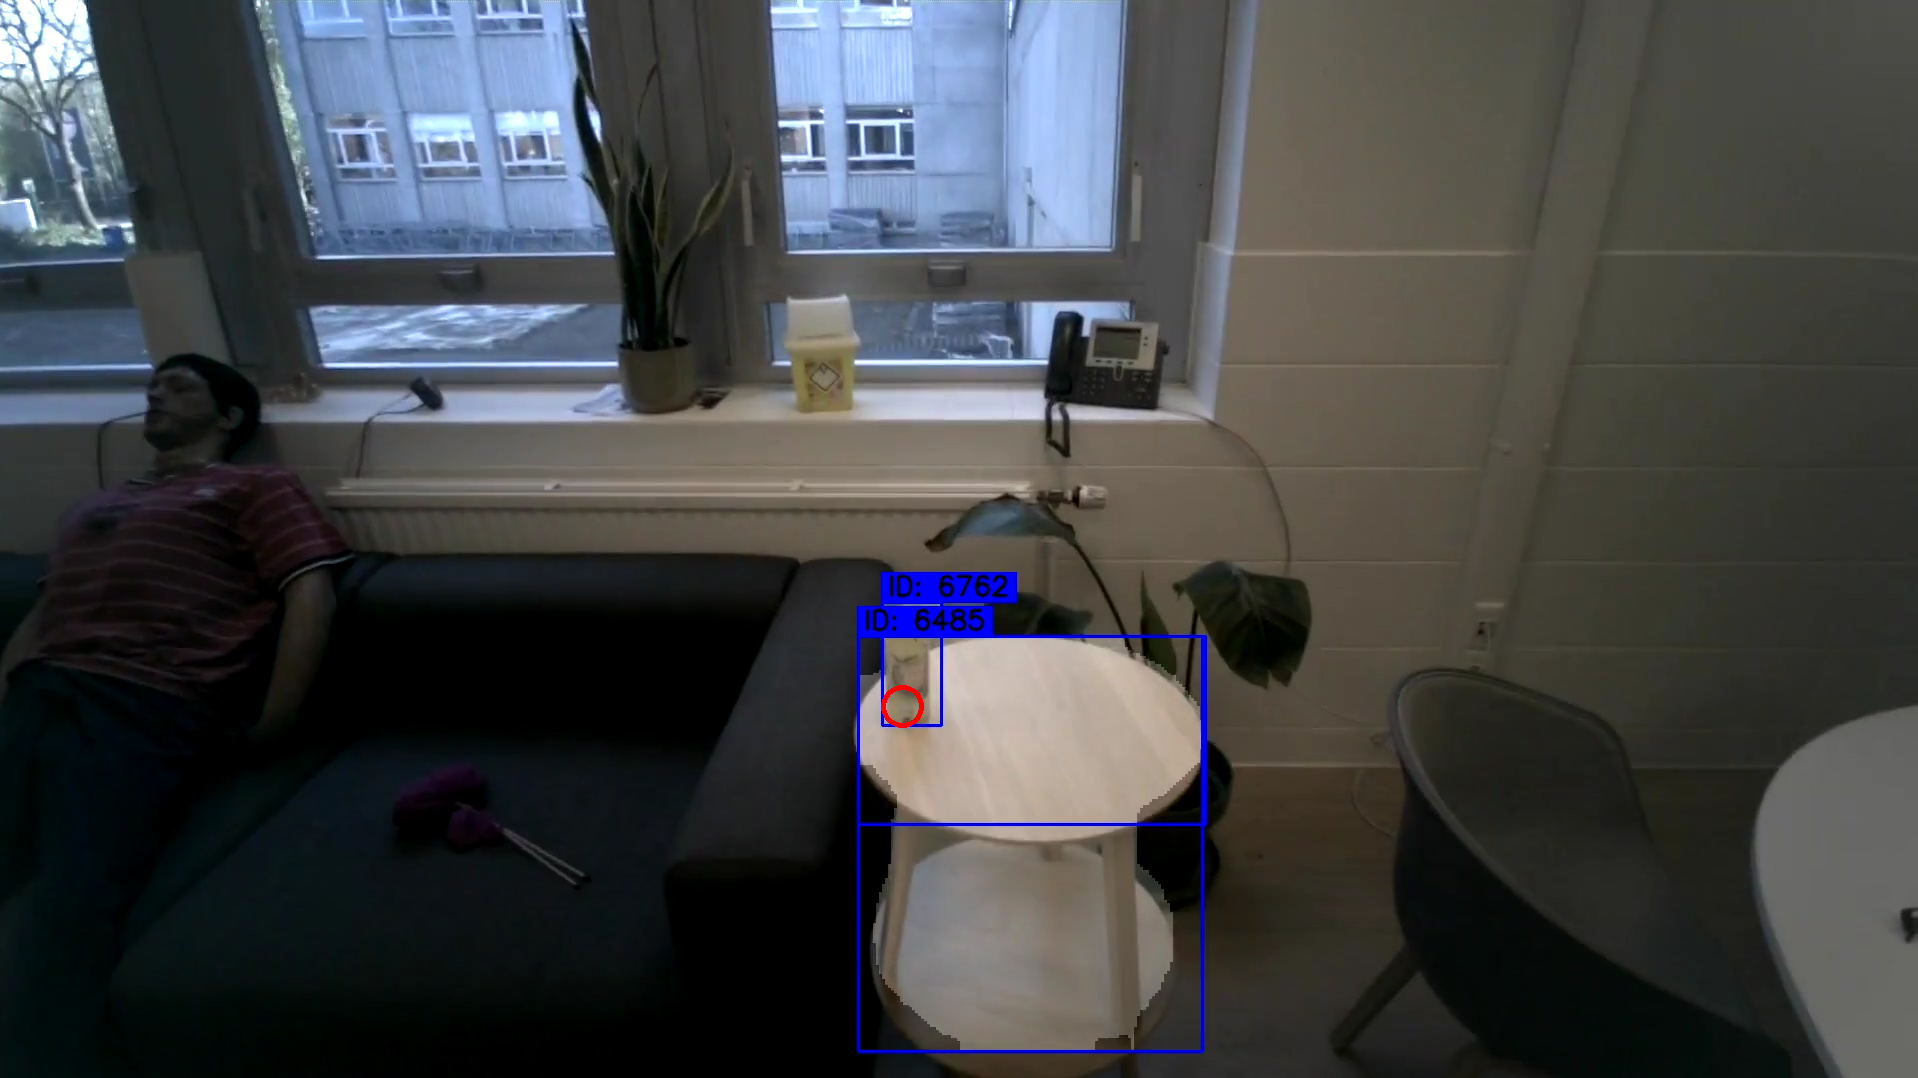
\includegraphics[width=1\textwidth]{filtered-segmentation.png}
    \caption{Filtering op basis van blikpunt en objectgrootte}
    \label{fig:pipeline_stap_b}
    \end{subfigure}

    \vspace{0.5cm}

    \begin{subfigure}[b]{0.75\textwidth}
        \centering
        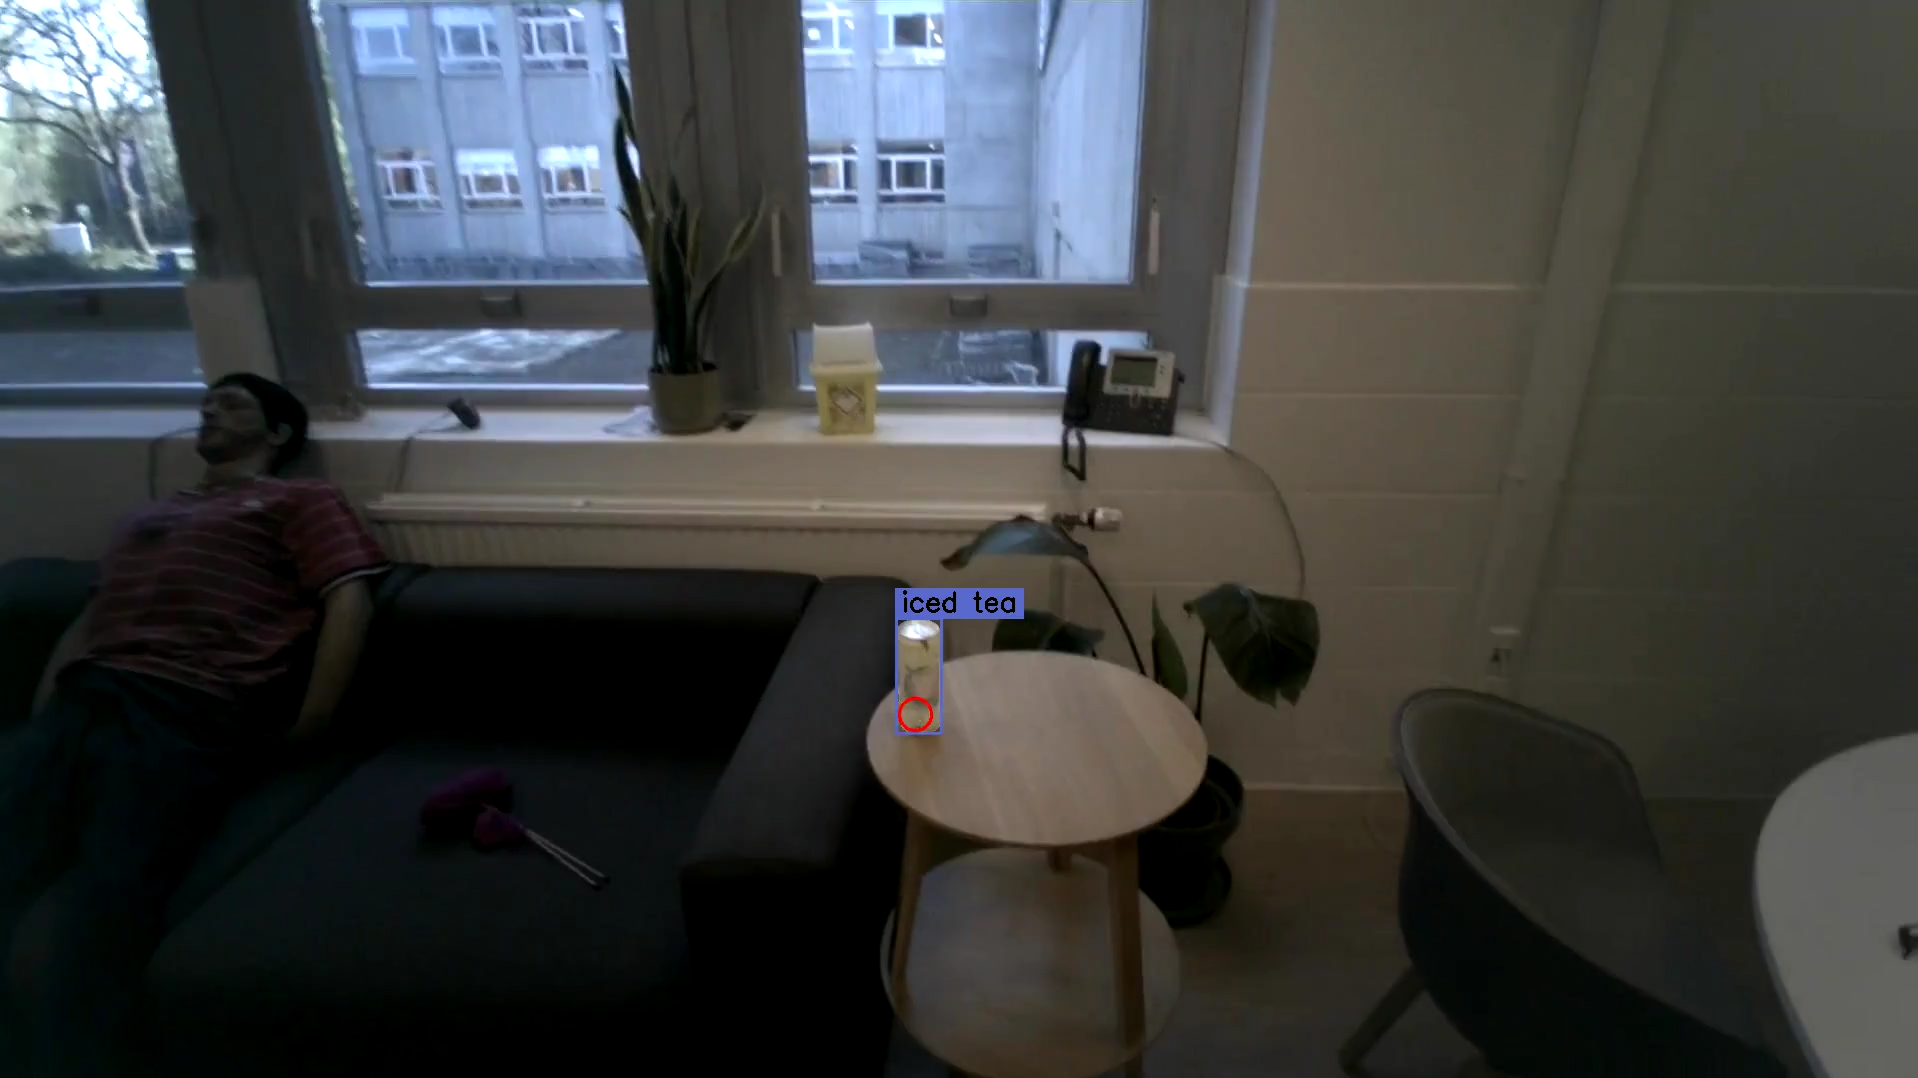
\includegraphics[width=1\textwidth]{classification-example.png}
        \caption{Classificatiestap}
        \label{fig:pipeline_stap_c}
    \end{subfigure}
    \caption[Visualisatie van de Analysepipeline]{
        \label{fig:analyse-pipeline-visualisatie}
        Visualisatie van de stappen in de analysepipeline.
        (\subref{fig:pipeline_stap_a}) FastSAM segmenteert alle objecten in het beeld en volgt deze doorheen de video.
        (\subref{fig:pipeline_stap_b}) De segmenten worden gefilterd; enkel de segmenten die daadwerkelijk met de blik van de gebruiker overlappen worden behouden.
        (\subref{fig:pipeline_stap_c}) De overgebleven segmenten worden uit de originele frame geknipt en dienen als input voor een classificatiemodel.
    }
\end{figure}

\section{Tracking en Segmentatie van Objecten}
\label{sec:tracking-segmentatie}

De eerste fase van de analysepipeline is erop gericht om uit de continue videostroom alle potentieel relevante objectregio's 
te isoleren die daadwerkelijk door de student zijn bekeken. 
De implementatie van dit proces werd vastgelegd in de python-notebook \texttt{04\_gaze\_segmentation.ipynb},
en wordt hieronder toegelicht.
De besproken code binnen deze fase is terug te vinden in de \texttt{GazeSegmentationJob} klasse in de notebook.

Voor deze fase werd gekozen om gebruik te maken van het FastSAM-model, vanwege zijn hoge snelheid.
Dit maakte het mogelijk om snel de aanpak te optimaliseren en de pipeline te testen, zonder dat de tijdsduur van de analyse een beperkende factor werd.
Het model komt in twee varianten: een `large' (\texttt{FastSAM-x}) en een `small' (\texttt{FastSAM-s}) versie.
Er werd gekozen om de `large' versie te gebruiken, vanwege de betere segmentatiekwaliteit.
FastSAM is beschikbaar via de \texttt{ultralytics}\footnote{\url{https://docs.ultralytics.com/models/fast-sam/} (laatst geraadpleegd op 2025-05-21)} python-bibliotheek,
die een \texttt{track} functie bevat die het mogelijk maakt om alle objecten in een video zowel te segmenteren als te tracken.

\subsection{Tracking en Segmentatie van Objecten}

In een eerste stap worden alle frames van de evaluatieopname geëxtraheerd naar een tijdelijke map met behulp van \texttt{ffmpeg}.
Daarna is het mogelijk om de \texttt{track} functie toe te passen op deze frames:

\begin{listing}[H]
  \begin{minted}{python}
    frame_paths = list(self.frames_path.iterdir())
    # Frames sorteren op basis van hun naam (index)
    frame_paths.sort(key=lambda x: int(x.stem))

    for frame_path in frame_paths:
        frame_idx = int(frame_path.stem)
        results = self.model.track(
            source=str(frame_path), imgsz=1024, verbose=False, persist=True
        )[0]
    \end{minted}
  \caption[Tracking van objecten met FastSAM]{}
\end{listing}

Hier zijn volgende zaken belangrijk om op te merken:
\begin{itemize}
    \item De frames dienen gesorteerd te worden op basis van hun volgorde in de video.
    \item De \texttt{track} functie neemt een parameter \texttt{imgsz} aan, die de grootte van de inputafbeeldingen bepaalt.
    Indien de afbeeldingen te groot of te klein zijn, worden ze automatisch geschaald.
    Deze parameter heeft zowel invloed op de snelheid van de segmentatie als op de kwaliteit ervan.
    \item Het is belangrijk om de \texttt{persist} parameter op \texttt{True} te zetten, 
    zodat het model de tracking-informatie kan behouden tussen opeenvolgende frames.
    \item De \texttt{track} functie levert een lijst op van \texttt{Results}-objecten, maar bevat hier slechts één element, aangezien de functie telkens een enkele frame behandelt.
    Dit \texttt{Results}-object bevat de segmentatiemaskers, bounding boxes, en tracking-informatie voor elk object in het frame.
\end{itemize}
Het is ook mogelijk om een \texttt{iou} (Intersection over Union) parameter in te stellen, evenals een \texttt{conf} (vertrouwensscore) parameter.
De \texttt{iou} parameter bepaalt hoeveel overlap nodig is tussen objecten om ze als hetzelfde object te beschouwen tijdens tracking.
Een hoge waarde zal meer objecten als verschillend beschouwen, terwijl een lage waarde meer objecten zal samenvoegen.
Echter werden deze parameters binnen dit onderzoek niet verder geoptimaliseerd.

\subsection{Filteren van Tracking-Resultaten}

Na het uitvoeren van de tracking en segmentatie, worden de resultaten gefilterd op basis van twee criteria:
\begin{itemize}
    \item \textbf{Objectgrootte:} Segmenten die een onrealistisch groot deel van het beeld beslaan (bijvoorbeeld muren, vloeren, of de gehele achtergrond) worden weggelaten.
    \item \textbf{Blikdata:} Met behulp van de \texttt{mask\_was\_viewed} functie (zie Sectie~\ref{sec:filtering-annotaties}) 
    wordt voor elk overgebleven segment gecontroleerd of het blikveld van de student daadwerkelijk overlapt met het segmentatiemasker in dat specifieke frame. 
    Enkel de `bekeken' segmenten worden behouden voor verdere analyse.
\end{itemize}

Hier zullen we enkel de \texttt{mask\_too\_large} functie toelichten.\\
Codefragment~\ref{listing:filteren-segmenten-grootte} toont de implementatie hiervan.

\begin{listing}[H]
  \begin{minted}{python}
    def mask_too_large(self, mask: torch.Tensor) -> bool:
        MAX_MASK_AREA = 0.1
        height, width = mask.shape
        frame_area = height * width
        max_mask_area = MAX_MASK_AREA * frame_area

        mask_area = mask.sum()
        return mask_area >= max_mask_area
    \end{minted}
  \caption[Filteren van segmenten op basis van grootte]{
    \label{listing:filteren-segmenten-grootte}  
    Deze functie controleert of een segment te groot is op basis van de oppervlakte van het segmentatiemasker. 
  }
\end{listing}

Hier wordt een som berekend van alle pixels in het segmentatiemasker (aangezien het masker binair is).
Indien deze som groter is dan de maximaal toegestane oppervlakte, wordt het masker als `te groot' beschouwd.
De maximale oppervlakte van een segment wordt gedefinieerd als 10\% van de totale oppervlakte van het frame.
Dit is momenteel een arbitraire waarde, maar kan in de toekomst verder geoptimaliseerd worden, of zelfs 
dynamisch worden ingesteld op basis van objecten binnen kalibratieopnames in de applicatie.

\subsection{Opslaan van de Resultaten}

Na het filteren van de segmenten, worden de resultaten van elke frame opgeslagen in gecomprimeerde numpy-bestanden 
(\texttt{.npz}) onder\\ \texttt{data/gaze\_segmentation\_results}.

\begin{listing}[H]
  \begin{minted}{python}
    executor.submit(
        np.savez_compressed,
        self.results_path / f"{frame_idx}.npz",
        boxes=boxes,
        rois=rois_array,
        masks=masks_array,
        object_ids=object_ids,
        frame_idx=frame_idx,
        gaze_position=gaze_position,
        confidences=confidences,
    )
    \end{minted}
  \caption[Opslaan van segmentatie-resultaten]{
    \label{listing:opslaan-segmentatie-resultaten}
    Deze code slaat de resultaten van de segmentatie en tracking op in een gecomprimeerd numpy-bestand.
    De resultaten worden opgeslagen per frame, met de relevante metadata.
  }
\end{listing}

De volgende gegevens worden opgeslagen:
\begin{itemize}
    \item \textbf{boxes:} De bounding boxes van de segmenten, handig voor het visualiseren van de segmenten in de video.
    \item \textbf{rois:} De ROI's (Region of Interest) van de segmenten. Deze worden later gebruikt bij de classificatiestap om de objecten te identificeren.
    \item \textbf{masks:} De segmentatiemaskers van de objecten, die ook worden gebruikt voor visualisatie.
    \item \textbf{object\_ids:} De unieke ID's van de objecten, die worden toegewezen door het FastSAM-model. Deze ID's blijven consistent voor elk specifiek object over meerdere frames,
    tenzij de tracking verloren gaat (bijvoorbeeld wanneer het object tijdelijk uit beeld is). Wanneer dit gebeurt, wordt een nieuwe ID toegewezen aan het object als het opnieuw in beeld komt.
    Deze ID maakt het mogelijk om de resultaten van de classificatiestap te aggregeren over meerdere frames, om zo een beter resultaat te krijgen.
    \item \textbf{frame\_idx:} De index van het frame, die wordt gebruikt om de resultaten te koppelen aan het juiste frame in de video.
    \item \textbf{gaze\_position:} De blikpositie van de student in dat specifieke frame (indien beschikbaar).
    \item \textbf{confidences:} De vertrouwensscore van het model voor elk segment, die aangeeft hoe zeker het model is dat het segment correct is.
    Dit kan nuttig zijn voor het filteren van segmenten die een lage vertrouwensscore hebben, 
    of het vinden van correlaties tussen de vertrouwensscore en de uiteindelijke classificatie.
\end{itemize}
Aangezien het opslaan van de resultaten IO-intensief is, wordt dit proces uitgevoerd met behulp van multithreading (\texttt{executor.submit}).

\subsection{Voorbereiding van de Tracking Resultaten voor Classificatie}
\label{sec:voorbereiding-tracking-resultaten}

De output van de vorige stap bestaat uit een reeks \texttt{.npz}-bestanden, één per frame, 
die de gefilterde segmenten, ROIs, en bijbehorende metadata bevatten. 
Om deze data efficiënt te kunnen gebruiken als input voor de classificatiestrategieën, werd een aanvullende voorbereidingsstap uitgevoerd. 
Deze stap werd geïmplementee\-rd in de notebook \texttt{05\_create\_object\_datasets.ipynb} en consolideert de frame-per-frame 
resultaten tot een gestructureerde dataset per evaluatieopname. 
Deze dataset, hierna `object-dataset' genoemd, aggregeert alle metadata van de bekeken segmenten binnen een enkele tabel.
Hoewel veel van deze metadata ook in de individuele \texttt{.npz}-bestanden te vinden zijn, resulteert de consolidatie 
naar één \texttt{.csv}-bestand per opname in een efficiëntere dataverwerking tijdens de classificatiefase. 
Het vermijdt het herhaaldelijk openen en parsen van potentieel honderden of duizenden afzonderlijke \texttt{.npz}-bestanden.

Het creëren van de object-dataset omvat het itereren over de \texttt{.npz}-bestanden van elke opname. 
Voor elk gedetecteerd en gefilterd object (ROI) binnen een frame worden de volgende kenmerken geëxtraheerd en samengevoegd tot een rij in een \texttt{Pandas DataFrame}:
\begin{itemize}
    \item \texttt{frame\_idx}: De index van het frame waarin het object oorspronkelijk werd gedetecteerd. 
    Dit koppelt het object aan een specifiek tijdstip in de video.
    \item \texttt{object\_id}: De unieke, tijdelijke ID die door het FastSAM-model aan het getrackte object 
    is toegewezen binnen de scope van die specifieke tracking-sessie.
    \item \texttt{confidence}: De vertrouwensscore van het FastSAM-model voor de detectie van dit specifieke segment. 
    Deze score geeft een indicatie van hoe zeker het model was van zijn segmentatie.
    \item \texttt{embedding}: Een dense vectorrepresentatie (embedding) van de visuele kenmerken van de ROI, 
    gegenereerd met het DINOv2-model. 
    Deze embedding dient als input voor de op similariteit gebaseerde classificatie met een vector-index.
    Meer hierover in de volgende sectie.
    \item \texttt{mask\_area}: De totale oppervlakte van het segmentatiemasker van het object in pixels. 
    Dit geeft een maat voor de (schijnbare) grootte van het object in het frame.
    \item \texttt{x1, y1, x2, y2}: De coördinaten die de bounding box rondom het gedetecteerde object definiëren. 
\end{itemize}

De resulterende \texttt{DataFrame} wordt vervolgens opgeslagen 
als een \texttt{.csv}-bestand onder \texttt{data/object\_datasets/<recording\_id>}. 
Het resultaat is een set van tabelvormige datasets die klaar zijn voor de daadwerkelijke classificatietaken.

\section{Classificatie van Objecten}

De vorige fase leverde een dataset op met bekeken objectsegmenten (ROIs) per evaluatieopname.
Deze kregen echter nog geen label toegewezen, dat aangeeft tot welk van de kritische objecten ze behoren.
Om dit te realiseren, werd een classificatiestap geïmplementeerd die de ROIs labelt op basis van hun visuele kenmerken.

\subsection{Data Labeling}

Voor het initialiseren en trainen van de classificatiestrategieën was het noodzakelijk om een dataset te hebben met gelabelde objecten.
Zoals eerder beschreven in Hoofdstuk~\ref{ch:experiment} (Sectie~\ref{sec:kalibratieopnames}), werden hiertoe 
twee specifieke kalibratieopnames gemaakt door de onderzoeker.
De eerste opname bevatte de objecten in hun oorspronkelijke posities en achtergrond, identiek aan de evaluatieopnames.
De tweede opname toonde dezelfde objecten tegen een significant afwijkende achtergrond, 
primair bedoeld om de invloed van contextvariatie te onderzoeken.

Bij de analyses die in dit hoofdstuk worden gepresenteerd, is uitsluitend gebruik gemaakt 
van de data uit de kalibratieopname met de originele achtergrond.
De beslissing om de tweede kalibratieopname buiten beschouwing te laten, werd genomen om de scope van deze bachelorproef beheersbaar te houden.
Een discussie over het potentieel van deze tweede dataset voor verder onderzoek is terug te vinden in Hoofdstuk~\ref{ch:conclusie}.

\paragraph{Labeling voor Classificatie}
Voor de initiële, op ROI-gebaseerde classificatiepogingen, was de labelingstrategie relatief eenvoudig.
Het volstond om voor elk van de objecten een representatief aantal ROIs te verzamelen en te labelen gedurende de 
tijdsvensters van 30 seconden waarin elk object centraal werd bekeken. 
Dit leverde voldoende voorbeelden van elk object op voor het trainen van de classificatiemodellen.

\paragraph{Labeling voor Objectdetectie}
Voor het trainen van het objectdetectiemodel was echter een meer omvattende aanpak vereist.
In tegenstelling tot ROI-classificatie die op geïsoleerde objectsegmenten werkt, wordt een objectdetector 
getraind om objecten te lokaliseren binnen een breder beeld.
Tijdens de training analyseert het model `crops' (vierkante regio's van het beeld) en leert het model om objecten te detecteren binnen zulke regio's.
Hierbij is het belangrijk dat binnen de labeling alle objecten in het beeld worden gemarkeerd, die potentieel binnen een crop kunnen vallen
(zie Figuur~\ref{fig:voorbeeld_crop_yolo_training} voor een conceptuele visualisatie van een crop).
De manier waarop deze crops worden gedefinieerd binnen de trainingsdataset, komt later in dit hoofdstuk aan bod.

\begin{figure}[H]
    \centering
    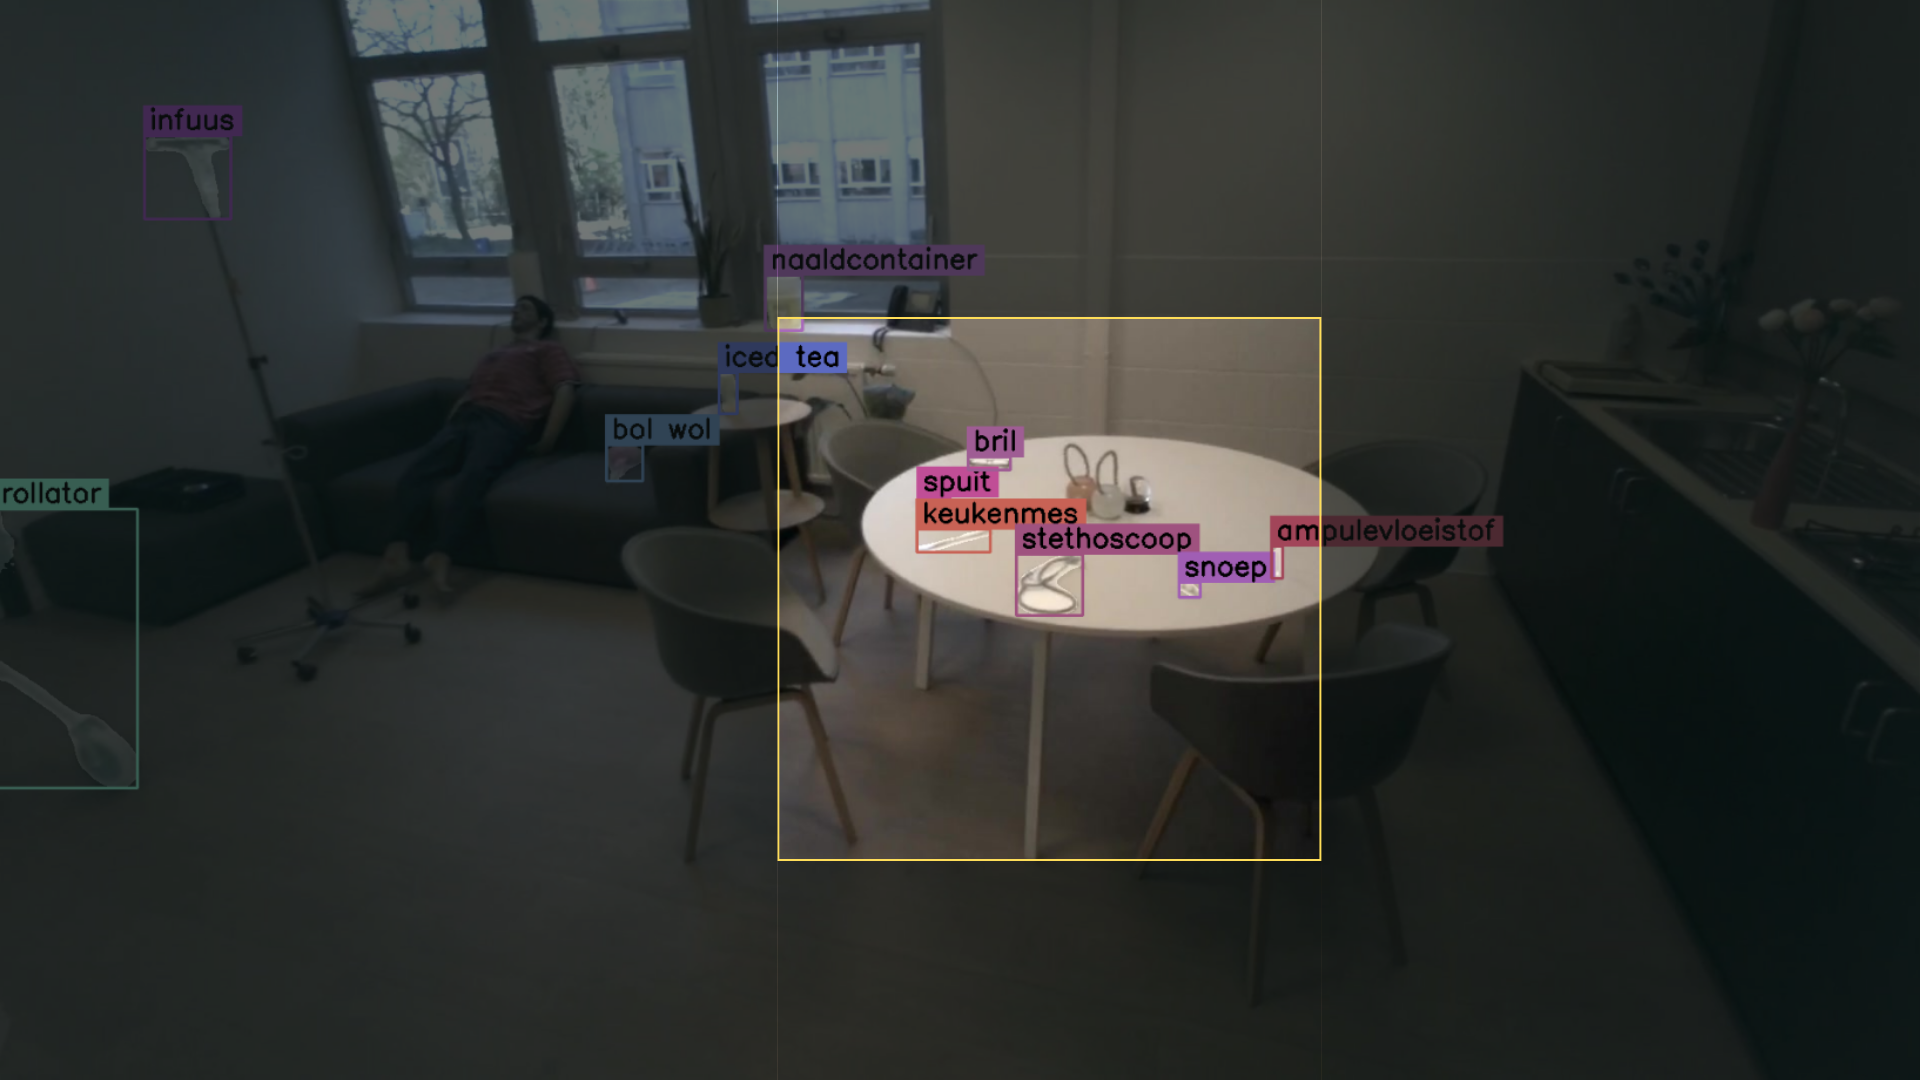
\includegraphics[width=1\textwidth]{yolo_training_crop.png}
    \caption[Voorbeeld van een crop voor objectdetectie]{
        \label{fig:voorbeeld_crop_yolo_training}
        Voorbeeld van een frame uit de labeling tool. 
        Hier wordt een voorbeeld van een crop getoond die gebruikt kan worden voor het trainen van een objectdetectiemodel.
        Het is dus belangrijk dat alle objecten die binnen deze crop kunnen vallen,
        worden gelabeld, zelfs als ze niet volledig zichtbaar zijn.
        Merk op dat dit niet de enige mogelijke crop is binnen deze afbeelding, men kan ook andere regio's selecteren met andere objecten.
    }
\end{figure}

\paragraph{Opmerking: Ampule Poeder Niet Gelabeld}
Het object `ampule poeder' werd in de labeling niet opgenomen. 
Origineel werd het object gekozen omwille van zijn doorschijnende karakter (glazen ampule).
Het werd ook naast een andere groep objecten geplaatst om de detectie alsnog te bemoeilijken (zie Figuur~\ref{fig:ampulepoeder}).
Echter, tijdens de labeling bleek het object te moeilijk voor het SAM2 model om te segmenteren en te tracken.
Dit resulteerde in een lage labelingkwaliteit, waarbij de segmenten inaccuraat waren.
Soms werden zelfs ook foutief, aangrenzende objecten meegenomen in de segmentaties.
Om deze reden werd besloten om het object niet mee te nemen in de labeling en de uiteindelijke analyse. 
Een ander object, de `ampule vloeistof', werd wel opgenomen ondanks zijn sterk doorschijnende karakter.
Dit object bleek veel gemakkelijker te volgen en te segmenteren door het FastSAM-model, vermoedelijk omdat het afgezonderd was van andere, 
potentieel verwarrende objecten.

\begin{figure}[H]
    \centering
    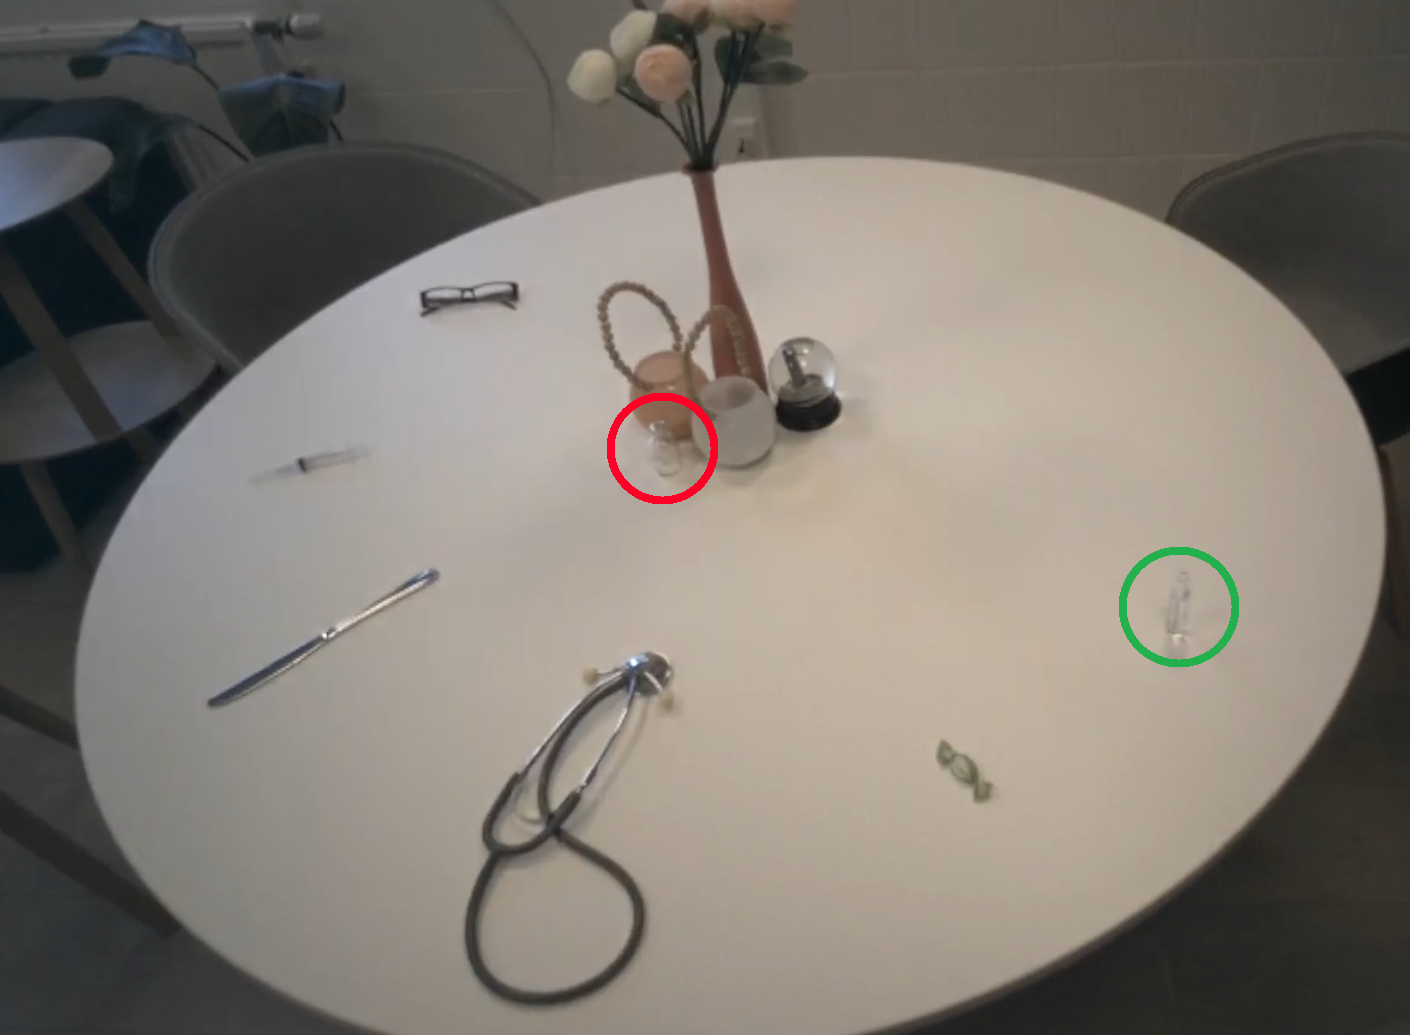
\includegraphics[width=0.8\textwidth]{ampulepoeder.png}
    \caption[Voorbeeld van de ampule poeder in de kalibratieopname]{
        \label{fig:ampulepoeder}
        Locatie van de ampule poeder in de kalibratieopname, aangeduid met een rode cirkel.
        De ampule vloeistof werd wel opgenomen in de labeling, en is hier aangeduid met een groene cirkel.
    }
\end{figure}

\subsection{Initiële Classificatiepogingen en Uitdagingen}

Nadat de object-datasets waren aangemaakt en de referentiedata uit de kalibratieopname was gelabeld, was de volgende stap het 
toewijzen van een label aan elk gedetecteerd en door de student bekeken objectsegment (ROI). 
Er werden initieel twee strategieën onderzocht voor het classificeren van deze ROIs, waarvan de relevante data beschikbaar waren in de object-datasets:
\begin{enumerate}
    \item \textbf{Vector-Index Classificatie:} Hierbij werden de DINOv2-embeddings van de ROIs vergeleken met referentie-embeddings van de kritische objecten afkomstig uit de kalibratieopname.
    Er werd een Faiss (Facebook AI Similarity Search) index gebruikt om de meest vergelijkbare referentie-embeddings te vinden.
    Faiss is een bibliotheek die het mogelijk maakt om snel zoekopdrachten uit te voeren op grote datasets van vectoren.
    \item \textbf{YOLOv11 Classificatie:} Een YOLO-model werd getraind, niet voor detectie in het volledige frame, maar specifiek voor het classificeren van de reeds 
    geïsoleerde ROIs uit de evaluatieopnames.
\end{enumerate}

Deze twee benaderingen zullen hier echter niet diepgaand worden behandeld, 
aangezien beiden al in een vroeg stadium van evaluatie een fundamenteel gebrek vertoonden, 
namelijk een onacceptabel hoge mate van vals-positieven. 
Het probleem lag niet zozeer in de specifieke modelkeuzes, maar in een verkeerde definitie van het classificatieprobleem.
De gekozen classificatietechnieken zijn inherent ontworpen voor \textit{gesloten-set} scenario's. 
In dergelijke scenario's  wordt aangenomen dat elke te classificeren input (elke bekeken ROI)
daadwerkelijk tot één van de vooraf gedefinieerde klassen behoort. 

De realiteit van de observaties is echter complexer en sluit veel beter aan bij het concept van \textit{Open Set Recognition (OSR)}. 
Zoals \textcite{Geng2018} beschrijven in hun overzichtsartikel, is het 
``doorgaans moeilijk om, wanneer men een herkenner of classificator traint, trainingsvoorbeelden te verzamelen die alle (mogelijke) klassen omvatten''.
OSR beschrijft een scenario waarin 
``er ten tijde van de training onvolledige kennis van de wereld bestaat, en onbekende klassen tijdens het testen aan een algoritme kunnen worden voorgelegd''.
Dit vereist dat een classificatiemodel ``niet alleen de geziene klassen accuraat classificeert, maar ook effectief omgaat met de ongeziene'' (citaten uit \textcite{Geng2018}, eigen vertaling).

In de context van dit onderzoek betekende dit dat de studenten talloze objecten en achtergrondelementen bekeken die \textit{niet} tot de kritische objecten behoorden.
De geïmplementeerde ROI-classificatiemodellen waren niet in staat om deze `onbekende' inputs effectief te herkennen en te verwerpen.
In plaats daarvan waren ze geneigd elke ROI te classificeren als één van de objecten, wat resulteerde in de waargenomen overvloed aan vals-positieven.

Gezien deze mismatch tussen de aard van het probleem en de gekozen aanpak, werd besloten deze classificatiestrategieën niet verder te optimaliseren.
De focus verschoof naar een methode die beter is uitgerust om specifieke, bekende objecten te identificeren: objectdetectie.

\section{Objectdetectie met YOLOv11} 

Bij de voorgaande classificatiestrategieën lag de focus op het classificeren van geïsoleerde objectsegmenten afkomstig uit de FastSAM everything-segmentatie.
Echter, de eerder beschreven problemen met vals-positieven maakten duidelijk dat een andere aanpak nodig was.
Objectdetectie biedt een krachtigere oplossing, omdat het niet alleen in staat is om objecten te classificeren, maar ook om hun locatie in het beeld te bepalen met behulp van bounding boxes.
De toegevoegde beeldcontext rond een object zorgt voor lagere gevoeligheid voor de problemen die zich voordeden bij de eerdere classificatiestrategieën.

\subsection{Creatie van de Trainingsdataset voor Objectdetectie}

Gebaseerd op de gelabelde kalibratieopname die eerder werd besproken, werd een specifieke trainingsdataset voor objectdetectie gecreëerd.
Zoals eerder vermeld, werd het object `ampule poeder' niet opgenomen in de labeling. Dit resulterende in een dataset met 14 objecten.
Deze diende te bestaan uit beelduitsnedes (hierna `crops' genoemd) waarin de kritische objecten gelabeld zijn met bounding boxes.
De creatie van deze dataset werd geïmplementeerd in de python notebook \texttt{12\_prepare\_object\_detection\_datasets.ipynb}.
Omwille van de beknoptheid zullen in deze sectie enkel de belangrijkste codefragmenten worden getoond; 
de geïnteresseerde lezer wordt verwezen naar de zonet vernoemde notebook voor de volledige implementatiedetails van de hieronder beschreven stappen.

\subsubsection{Formaat van de Trainingsdataset}

Alvorens de trainingsdataset te creëren, was het belangrijk om het beoogde formaat van de dataset te bepalen.
Een eerste overweging was de resolutie van de crops. 
Om tot een geïnformeerde keuze te komen, werd een analyse uitgevoerd op de afmetingen van de bounding boxes 
van de gelabelde objecten in de kalibratieopname. 
Figuur~\ref{fig:size-histogram} toont histogrammen van zowel de breedte (links) als de hoogte (rechts) 
in pixels van deze bounding boxes. 
Uit de histogrammen blijkt dat de meerderheid van de objecten een breedte en hoogte hebben van minder dan 400 pixels. 
Enkele objecten die van zeer dichtbij waren opgenomen, vertoonden grotere afmetingen. 
Op basis van deze observatie, en rekening houdend met het feit dat objecten in de praktijk 
niet altijd perfect in het midden van een crop zullen liggen, 
werd gekozen voor een vierkante crop-grootte van 640x640 pixels. 
Deze afmeting biedt een ruime marge om de meeste objecten volledig te omvatten, zelfs als ze enigszins 
verschoven zijn ten opzichte van het centrum van de crop. 
Deze grootte is tevens een gangbare inputresolutie voor YOLO-modellen.

\begin{figure}[H]
    \centering
    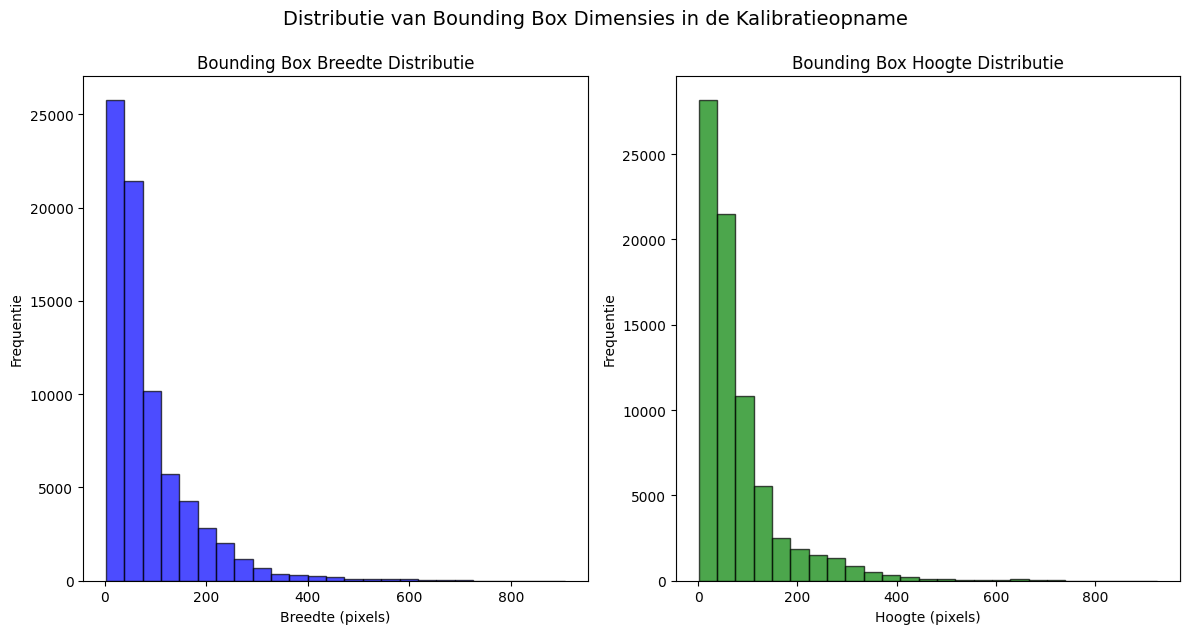
\includegraphics[width=1\textwidth]{bboxes-histogrammen.png}
    \caption[Histogrammen van de breedte en grootte van bounding boxes in de kalibratieopname]{
      \label{fig:size-histogram}
      Histogrammen van de breedte (links) en hoogte (rechts) in pixels van de bounding boxes in de kalibratieopname.
      De meeste objecten waren minder dan 400 pixels in zowel breedte als hoogte, met een aantal uitzonderingen.
    }
\end{figure}

De volgende overweging betrof de wijze waarop deze crops gegenereerd zouden worden uit de kalibratieopname. 
Aangezien het uiteindelijke doel was om de ROIs die gegenereerd werden door FastSAM, te classificeren, 
dient de trainingsdataset zo goed mogelijk de karakteristieken van deze te classificeren ROIs te weerspiegelen. 
In de praktijk zullen deze ROIs vaak (maar niet altijd perfect) gecentreerd zijn rond het blikpunt van de student, 
omdat de FastSAM-segmentatie en de blikpuntfiltering hierop aansturen. 
Daarom werd voor de creatie van de trainingsdataset besloten om de crops te genereren 
door ze te centreren op het middelpunt van de bounding box van een \textit{geselecteerd doelobject} uit de kalibratieopname. 
Dit simuleert de situatie waarbij het model een ROI aangeboden krijgt waarin het doelobject centraal staat.

Tenslotte vereiste de trainingsdataset voor objectdetectie ook een specifieke structuur, zijnde het 
\textit{Ultralytics YOLO formaat}\footnote{\url{https://docs.ultralytics.com/datasets/detect/\#ultralytics-yolo-format} (laatst geraadpleegd op 2025-05-21).} (zie Codefragment~\ref{fig:yolo-format}).

\begin{listing}[H]
  \begin{minted}{text}
    data/
    ├── images/
    │   ├── train/
    │   │   ├── 0000000001.jpg
    │   │   ├── 0000000002.jpg
    │   │   ├── 0000000003.jpg
    │   │   └── ...
    │   └── val/
    │       ├── 0000000001.jpg
    │       ├── 0000000002.jpg
    │       ├── 0000000003.jpg
    │       └── ...
    ├── labels/
    │   ├── train/
    │   │   ├── 0000000001.txt
    │   │   ├── 0000000002.txt
    │   │   ├── 0000000003.txt
    │   │   └── ...
    │   └── val/
    │       ├── 0000000001.txt
    │       ├── 0000000002.txt
    │       ├── 0000000003.txt
    │       └── ...
    └── data.yml
  \end{minted}
  \caption[Voorbeeld van het Ultralytics YOLO Formaat]{
    \label{fig:yolo-format}
    Voorbeeld van de structuur van de trainingsdataset voor objectdetectie in het Ultralytics YOLO formaat.
    De dataset bestaat uit een map met afbeeldingen (in dit geval crops) en een map met labels.
    Elke afbeelding heeft een bijbehorend labelbestand met dezelfde naam, waarin de bounding boxes en klassenamen van elk object in de afbeelding zijn gedefinieerd.
    Het \texttt{data.yml} bestand bevat de metadata van de dataset. Dit komt later aan bod.
  }
\end{listing}

\subsubsection{Genereren van de Trainingsdataset}

Het eigenlijke proces voor het creëren van de trainings- en validatiedatasets werd gecoördineerd door de functie \texttt{create\_dataset} 
(zie Codefragment~\ref{listing:create-dataset-overview}). 
Deze functie neemt de metadata van de gelabelde objecten, de geëxtraheerde frames van de kalibratieopname 
en de configuratieparameters zoals de crop-grootte en het gewenste aantal samples per klasse, als input.

\begin{listing}[H]
  \fontsize{10pt}{9.6pt}
  \begin{minted}{python}
  def create_dataset(
      per_class_metadata: dict,
      frames: list[Path],
      datasets_path: Path,
      crop_size: int,
      dataset_type: str,
      num_samples_per_class: int,
  ):
      # Definieren van de paden voor de trainings- en validatiedatasets
      # ... Code weggelaten voor beknoptheid ...

      # Samples selecteren per klasse en train/val splitsen
      selected_samples_per_class = select_samples_per_class(
          per_class_metadata, num_samples_per_class
      )
      all_samples_per_frame = get_samples_per_frame(per_class_metadata)
      train_samples_per_class, val_samples_per_class = get_train_val_split(
          selected_samples_per_class, train_ratio=0.8
      )

      # Datasetfiles aanmaken
      class_label_to_model_id = create_metadata_yaml(dataset_path, per_class_metadata)
      create_train_or_val_dataset(
          per_class_metadata,
          class_label_to_model_id,
          train_samples_per_class,
          all_samples_per_frame,
          frames,
          train_images_path,
          train_labels_path,
          crop_size=crop_size,
      )
      create_train_or_val_dataset(
          per_class_metadata,
          class_label_to_model_id,
          val_samples_per_class,
          all_samples_per_frame,
          frames,
          val_images_path,
          val_labels_path,
          crop_size=crop_size,
          is_validation=True,
      )

      return dataset_path
  \end{minted}
  \caption[Functie voor het creëren van de objectdetectie-trainingsdataset]{
    \label{listing:create-dataset-overview}
    De \texttt{create\_dataset} functie coördineert het creëren van de trainings- en validatiedatasets voor objectdetectie.
    Deze functie definieert de paden voor de datasets, maakt de benodigde mappen aan,
    selecteert de samples per klasse, splitst deze in train- en validatiesets
    en roept de \texttt{create\_train\_or\_val\_dataset} functie aan om de crops en labels te genereren. 
  }
\end{listing}

De benodigde stappen voor het creëren van de trainingsdataset kunnen worden samengevat in drie hoofdfasen, zoals hieronder beschreven.

\paragraph{1. Verzamelen van Metadata per Klasse}

De notebook laadt in een eerste stap de bestandspaden van de trackingresultaten per klasse 
voor de kalibratieopname via de functie\\ \texttt{get\_tracking\_results\_per\_class}.\\
Vervolgens worden op basis van de trackingresultaten, metadata per klasse verzameld door de functie \texttt{get\_metadata\_per\_class} aan te roepen.
Dit resulteert in een dictionary waarin elke klasse ID is gekoppeld aan een dictionary met de volgende informatie:
\begin{itemize}
    \item \texttt{class\_name}: De naam van de klasse, bijvoorbeeld `monitor'.
    \item \texttt{color}: Het kleur van de klasse in hexadecimale notatie.
    \item \texttt{frame\_indexes}: Een lijst van frame-indexen waarin de klasse voorkomt in de trackingresultaten.
    \item \texttt{mask\_areas}: Een lijst van de oppervlakte van het segmentatiemasker voor elk frame waarin de klasse voorkomt.
    \item \texttt{bboxes}: Een lijst van bounding boxes voor elk frame waarin de klasse voorkomt.
\end{itemize}
Elke combinatie van een frame-index en bijbehorende bounding box uit deze lijsten representeert 
een uniek gelabeld voorbeeld (een `sample') van een object in de kalibratieopname.

Figuur~\ref{fig:samples-per-class} toont het aantal verzamelde samples per klasse in de kalibratieopname. 
Aangezien sommige objecten dichter bij elkaar stonden, 
zijn er voor die objecten meer samples verzameld dan voor andere.
Zo zien we dat het infuus relatief weinig samples heeft, omdat het in een afgezonderde hoek van het beeld stond.
Hierdoor zijn er enkel samples verzameld binnen de 30 seconden waarin het infuus werd bekeken, 
of wanneer het zichtbaar was in de achtergrond.

\begin{figure}[H]
    \centering
    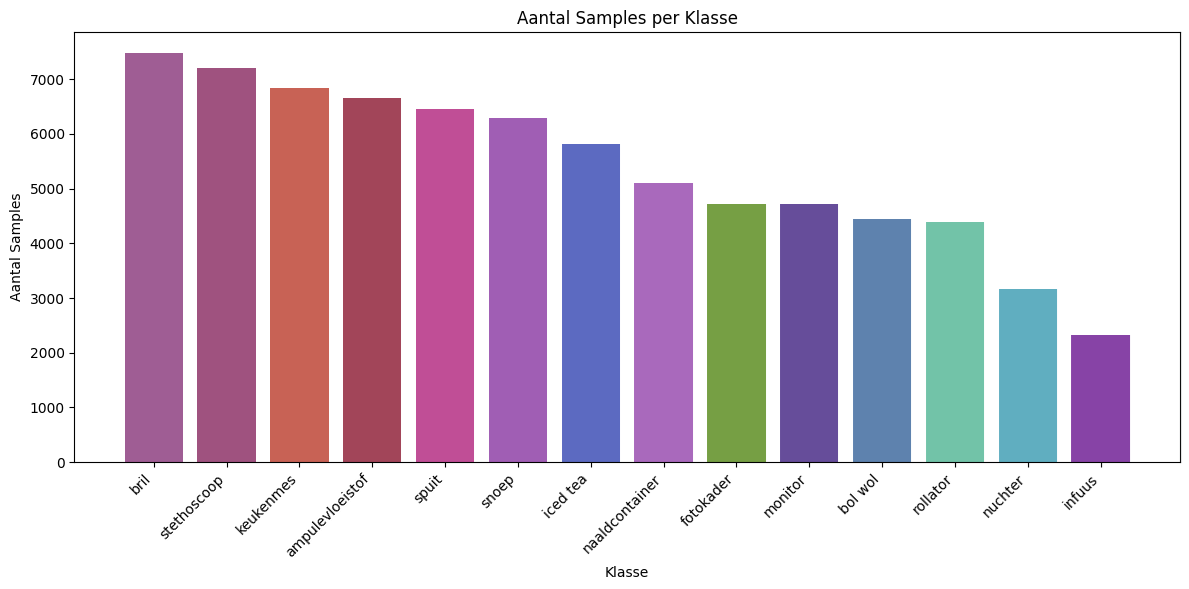
\includegraphics[width=1\textwidth]{samples-per-class.png}
    \caption[Aantal samples per klasse in de kalibratieopname]{
        \label{fig:samples-per-class}
        Aantal samples per klasse in de kalibratieopname.
        De getoonde aantallen zijn het resultaat van de tracking binnen de labeling tool.
      }
\end{figure}

De \texttt{per\_class\_metadata} dictionary werd vervolgens doorgegeven aan de\\ \texttt{create\_dataset} functie.
Elke dataset werd opgeslagen in de map\\ \texttt{data/training\_datasets/object\_detection}.

\paragraph{2. Selectie van Voorbeeldsamples per Klasse}
Om een gebalanceerde dataset te creëren voor training, en om de impact van de datasetgrootte te kunnen onderzoeken, 
werd per objectklasse een specifiek aantal voorbeeld-samples geselecteerd. 
De functie \texttt{select\_samples\_per\_class} implementeert deze selectie. 
Er werd geëxperimenteerd met verschillende aantallen samples per klasse: 500, 1000, 2000 en 3000 via de parameter \texttt{num\_samples\_per\-\_class}.
Indien een klasse onvoldoende unieke samples bevatte ten opzichte van het opgegeven aantal, werd oversampling toegepast.
Alle beschikbare unieke samples werden eerst geselecteerd, waarna de resterende samples willekeurig met vervanging uit de beschikbare pool werden getrokken.

Met deze mapping werden de train- en validatiesets gedefinieerd.
De functie\\ \texttt{get\_train\_val\_split} verdeelt de geselecteerde samples in een train- en validatieset,
met een splitsing van 80\% voor training en 20\% voor validatie.
Deze stap resulteerde in twee mappings: \texttt{train\_samples\_per\_class} en \texttt{val\_samples\_per\_class}.

Tenslotte werd ook per frame een lijst van \textit{alle} (dus niet enkel de geselecteerde) bounding boxes verzameld.
Dit is van belang omdat bij het maken van een crop rond een \textit{geselecteerd doelobject},
ook alle \textit{andere} objecten die toevallig in die crop vallen, correct voorspeld moeten worden door de objectdetector.
De functie \texttt{get\_samples\_per\_frame} creërde hiertoe een dictionary\\ \texttt{all\_samples\_per\_frame}, 
waarbij elke frame-index gemapt werd naar een lijst van alle objecten (klasse-ID en bounding box) die in dat frame voorkomen.

\paragraph{3. Genereren van Crops en YOLO-Labels voor Trainings- en Validatiesets}
Met de voorbereide lijsten van geselecteerde trainings- en validatiesamples per 
klasse (\texttt{train\_samples\_per\_class} en \texttt{val\_samples\_per\_class}) 
en de complete lijst van alle gelabelde objecten per frame (\texttt{all\_samples\_per\_frame}), 
kon de daadwerkelijke generatie van de dataset beginnen. 
Dit proces werd uitgevoerd door de functie \texttt{create\_train\_or\_val\_dataset}, 
die afzonderlijk werd aangeroepen voor het creëren van de trainingsdata en de validatiedata. 
De functie \texttt{create\_dataset} fungeerde als een overkoepelende wrapper die de mappenstructuur 
aanmaakte en de \texttt{create\_train\_or\_val\_dataset} functie aanriep.

\begin{listing}[H]
  \fontsize{11pt}{9.6pt}
  \begin{minted}{python}
    def create_train_or_val_dataset(
      per_class_metadata,
      class_label_to_model_id,
      selected_samples_per_class,
      all_samples_per_frame,
      frames,
      images_path,
      labels_path,
      crop_size: int,
      is_validation=False,
  ):
      selected_samples_per_frame = get_selected_samples_per_frame(
          selected_samples_per_class
      )

      current_sample_idx = 0
      for frame_idx, frame in enumerate(tqdm(frames)):
          if selected_samples_per_frame.get(frame_idx) is None:
              continue

          image = cv2.imread(str(frame))

          # verzamelen van alle bounding boxes en klassenamen in de huidige frame
          class_ids, bboxes = zip(*all_samples_per_frame[frame_idx])
          bboxes = np.array(bboxes)
          class_labels = [
              per_class_metadata[class_id]["class_name"] for class_id in class_ids
          ]

          # aanmaken van de crops voor elk geselecteerd doelobject in de huidige frame
          for _, target_box in selected_samples_per_frame[frame_idx]:
              transformed_image, transformed_bboxes, transformed_class_labels = create_crop_for_frame(
                  image,
                  crop_size,
                  target_box,
                  bboxes,
                  class_labels,
                  is_validation
              )

              create_data_files(
                  labels_path,
                  images_path,
                  class_label_to_model_id,
                  current_sample_idx,
                  transformed_image,
                  transformed_bboxes,
                  transformed_class_labels,
              )

              current_sample_idx += 1
  \end{minted}
  \caption[Functie voor het creëren van de trainings- en validatiedatasets]{
    \label{listing:create-train-val-dataset}
    De \texttt{create\_train\_or\_val\_dataset} functie genereert de crops en labels voor de trainings- of validatiedataset.
    Het laadt de originele afbeelding, verzamelt de relevante bounding boxes en klassenamen 
    en maakt voor elk geselecteerd doelobject een crop rond de bounding box.
    }
\end{listing}

De werking van \texttt{create\_train\_or\_val\_dataset} is als volgt:
\begin{enumerate}
    \item Eerst worden de \texttt{selected\_samples\_per\_class} (die de geselecteerde doelobjecten voor de huidige set bevatten) 
    geherstructureerd naar een per-frame dictionary \texttt{selected\_samples\_per\_frame}.
    \item De functie itereert vervolgens over alle frames van de kalibratieopname.
    \item Voor elke frame wordt de originele afbeelding geladen indien er samples voor die frame zijn geselecteerd. 
    Ook worden alle bounding boxes en bijbehorende klassenamen van 
    \textit{alle} gelabelde objecten in die frame verzameld uit \texttt{all\_samples\_per\_frame}.
    \item Daarna wordt geïtereerd over elk \textit{geselecteerd doelobject}
    dat in de huidige frame aanwezig is (opgehaald uit \texttt{selected\_samples\_per\_frame}). 
    Het is rond deze \texttt{target\_box} dat een crop zal worden gemaakt.
    \item Voor elk \texttt{target\_box} binnen de frame wordt de functie\\ \texttt{create\_crop\_for\_frame} aangeroepen. 
    Deze functie, hieronder beschreven, retourneert de beelduitsnede. Het geeft tevens de bounding boxes, en de klassenamen 
    weer van alle objecten die na het croppen nog significant zichtbaar zijn binnen die uitsnede.
    \item Tenslotte worden de resultaten opgeslagen via de hulpfunctie \texttt{create\_data\-\_files},
    die de beelduitsnede en de bijbehorende labels opslaat in de juiste mappenstructuur.
\end{enumerate}

De functie \texttt{create\_crop\_for\_frame} in Codefragment~\ref{listing:create-crop-frame} 
is verantwoordelijk voor het creëren van de crop rond het doelobject.
Het transformeert ook de bounding box-coördinaten van alle relevante objecten naar het coördinatenstelsel van de\\ nieuwe crop 
en past indien nodig augmentaties toe.

\begin{listing}[H]
  \fontsize{11pt}{10pt}
  \begin{minted}{python}
    def create_crop_for_frame(
        image: np.ndarray,
        crop_size: int,
        target_box: tuple[int, int, int, int],
        bboxes: np.ndarray,
        class_labels: list[str],
        is_validation: bool = False,  
    ):
        x1, y1, x2, y2 = target_box
        cx, cy = (x1 + x2) // 2, (y1 + y2) // 2

        # crop aanmaken rond het doelobject
        half_crop = crop_size // 2
        x_min = max(0, cx - half_crop)
        y_min = max(0, cy - half_crop)
        x_max = min(image.shape[1], cx + half_crop)
        y_max = min(image.shape[0], cy + half_crop)

        transform_steps = [
            A.Crop(x_min=x_min, y_min=y_min, x_max=x_max, y_max=y_max),
            A.PadIfNeeded(min_height=crop_size, min_width=crop_size),
        ]

        if not is_validation:
            transform_steps.append(A.HorizontalFlip(p=0.5))
            transform_steps.append(
                A.RandomBrightnessContrast(p=0.2)
            )

        transform = A.Compose(
            transform_steps,
            bbox_params=A.BboxParams(
                format="pascal_voc", label_fields=["class_labels"], min_visibility=0.7
            ),
        )

        # augmenteren van de afbeelding en herberekenen van de bounding boxes
        augmented = transform(image=image, bboxes=bboxes, class_labels=class_labels)
        transformed_image = augmented["image"]
        transformed_bboxes = augmented["bboxes"]
        transformed_class_labels = augmented["class_labels"]
        return transformed_image, transformed_bboxes, transformed_class_labels
  \end{minted}
  \caption[Functie voor het creëren van een crop rond een doelobject]{
    \label{listing:create-crop-frame}
    De \texttt{create\_crop\_for\_frame} functie maakt een crop rond een doelobject in de afbeelding.
    Het past ook transformaties en augmentaties toe, al naar gelang de crop bedoeld is voor training of validatie.
    De functie retourneert de getransformeerde afbeelding, de bounding boxes, en de klassenamen van de objecten in de crop.
    }
\end{listing}

Voor het uitvoeren van beeldtransformaties en augmentaties werd de open-source bibliotheek \texttt{Albumentations} gebruikt \autocite{Buslaev2018}.
De bibliotheek staat toe om eenvoudig transformatiepipelines te definiëren en vereenvoudigt sterk het werken met bounding-box coördinaten.
Augmentaties kunnen de robuustheid van een model verbeteren door extra variatie aan de trainingsdata toe te voegen.
De volgende transformaties en augmentaties werden toegepast:
\begin{itemize}
    \item \textbf{\texttt{A.Crop}}: Deze transformatie werd gebruikt om een vierkante uitsnede te maken rond het geselecteerde doelobject.
    \item \textbf{\texttt{A.PadIfNeeded}}: Soms kan het zijn dat de crop deels buiten de grenzen van de originele afbeelding valt.
    Om dit te voorkomen, wordt padding met nullen toegepast om de crop altijd te vullen tot de gewenste grootte.
    \item \textbf{\texttt{A.HorizontalFlip}}: Deze augmentatie wordt willekeurig toegepast met een kans van 50\% om de afbeelding horizontaal te spiegelen.
    \item \textbf{\texttt{A.RandomBrightnessContrast}}: Deze augmentatie past willekeurig de helderheid en het contrast van de afbeelding aan met een kans van 20\%.
\end{itemize}
De transformaties \texttt{A.Crop} en \texttt{A.PadIfNeeded} werden altijd toegepast,
terwijl de transformaties \texttt{A.HorizontalFlip} en \texttt{A.RandomBrightnessContrast} 
enkel werden toegepast als een crop bedoeld was voor de trainingset (dus niet voor de validatieset).
Het toepassen van de \texttt{A.Crop} transformatie paste ook de bounding box coördinaten aan van frame-niveau naar crop-niveau.
Tenslotte heeft de \texttt{A.BboxParams} parameter ook een \texttt{min\_visibility} parameter, die ervoor zorgt dat alleen bounding boxes
met een zichtbaarheid van minstens 70\% worden behouden in de crop.
Deze parameter werd hardgecodeerd op 70\%, maar kan in de toekomst, indien nodig, verder geoptimaliseerd worden.

\subsection{Training van YOLOv11 Modellen}

Met de aangemaakte trainingsdatasets, kon de volgende stap beginnen: het trainen van YOLOv11-modellen.
Zoals eerder vermeld, werden vier verschillende datasets gecreëerd, elk met een ander aantal samples per klasse: 500, 1000, 2000 en 3000.
Voor elke dataset werd een afzonderlijk model getraind.

Voor de training werd gebruik gemaakt van het \texttt{YOLOv11n.pt} model. 
Dit is de `nano'-variant van een reeks modellen die zijn voorgetraind (volgens \textcite{Khanam2024}) op de COCO-dataset.
Het starten met een voorgetraind model is een gangbare praktijk in transfer learning, waarbij het model 
al een basisniveau van kennis heeft over objectherkenning.
Hiermee kan het model sneller convergeren met een kleinere dataset aan domeinspecifieke objecten, dan wanneer training aangevat wordt vanaf nul.

De training werd uitgevoerd met behulp van de functionaliteit van de \texttt{ultralytics}\footnote{\url{https://pypi.org/project/ultralytics/} (laatst geraadpleegd op 2025-05-29)} bibliotheek, 
binnen de script \texttt{scripts/train\_object\_detectors.py}.
De relevante code voor het trainen van de modellen is te vinden binnen de functie\\ \texttt{train\_model} in Codefragment~\ref{listing:train-model}.

\begin{listing}[H]
  \begin{minted}{python}
    TRAIN_EPOCHS = 100
    BATCH_SIZE = 0.9
    PATIENCE = 10

    def train_model(dataset_path, model_name, crop_size):
        model = YOLO("yolo11n.pt")

        model.train(
            data=dataset_path / "data.yaml",
            epochs=TRAIN_EPOCHS,
            imgsz=int(crop_size),
            device="cuda",
            batch=BATCH_SIZE,
            patience=PATIENCE,
            plots=True,
            save=True,
        )

        model_path = OBJECT_DETECTION_MODELS_PATH / f"{model_name}.pt"
        model.save(str(model_path))
    }
  \end{minted}
  \caption[Functie voor het trainen van YOLOv11-modellen]{
    \label{listing:train-model}
    De \texttt{train\_model} functie traint een YOLOv11-model op basis van de opgegeven dataset.
    Het gebruikt een voorgetraind model (\texttt{yolo11n.pt}) en past de training toe op de opgegeven dataset voor een bepaald aantal epochs.
    De \texttt{patience} parameter bepaalt hoeveel epochs het model zonder verbetering mag trainen.
  }
\end{listing}

Voor de training werden de volgende hyperparameters gebruikt:
\begin{itemize}
    \item \textbf{Epochs:} 100 epochs, wat betekent dat het model de volledige dataset 100 keer doorloopt.
    \item \textbf{Batch Size:} 0.9, wat betekent dat de batchgrootte automatisch wordt berekend om 90\% van het beschikbare GPU-geheugen te gebruiken. 
    \item \textbf{Patience:} Een patience van 10 betekent dat de training stopt als er gedurende 10 opeenvolgende epochs geen verbetering in de validatieprestaties wordt waargenomen.
    Aangezien de prestaties van de modellen tijdens de training echter steeds beter werden tot en met de 100ste epoch, werd de training niet vroegtijdig gestopt.
\end{itemize}
De \texttt{train\_model} functie werd telkens in een apart proces uitgevoerd voor optimalisatie van het geheugenbeheer.
Tenslotte werd elk model opgeslagen in de map \texttt{data/models/object\_detection}.

\subsection{Combineren van Objectdetectie en FastSAM Tracking}

Met de getrainde modellen was het mogelijk om de objectdetectie te koppelen aan de eerder verkregen FastSAM trackingresultaten uit Sectie~\ref{sec:tracking-segmentatie}.
In deze sectie wordt het proces beschreven om de FastSAM segmentaties te combineren met objectdetectie,
met als doel een dataset te verkrijgen die voor elke frame van de evaluatieopnames een lijst aan gelabelde, bekeken objecten bevat.
Het proces werd geïmplementeerd in de notebook \texttt{13\_predict\_object\_detection.ipynb} en kan worden samengevat in de volgende stappen:
\begin{enumerate}
    \item \textbf{Genereren van Vergelijkingssets per Frame}: Voor elke frame van een evaluatieopname werd een 
    `vergelijkingsset' samengesteld. 
    Deze set bracht de informatie uit twee bronnen samen. 
    De eerste component bestond uit de door FastSAM geïdentificeerde objectsegmenten, 
    die al eerder op basis van de blikdata van de student waren geselecteerd. 
    De tweede component bevatte de objectdetecties die het resultaat waren van de toepassing van het getrainde 
    YOLOv11-model op een specifieke uitsnede (crop) binnen het betreffende frame. 
    Deze uitsnede werd gecentreerd rond het blikpunt van de student.
    \item \textbf{Matchen van Segmentaties en Detecties:} 
    Binnen elke vergelijkingsset werden de FastSAM-segmentaties gematcht met de YOLOv11-detecties op 
    basis van ruimtelijke overlap (Intersection over Union, IoU), waarbij enkel betrouwbare matches werden behouden.
    De term `Intersection over Union' wordt in de volgende sectie verder toegelicht.
    \item \textbf{Toekennen van een Klasse aan FastSAM Object Tracks:} 
    De klassevoorspellingen van de gematchte YOLOv11-detecties werden geaggregeerd voor elke unieke FastSAM object ID 
    (die een object over meerdere frames volgt). 
    Op basis hiervan werd een definitieve classificatie (één van de 14 kritische objecten of 'onbekend') 
    toegekend aan elke FastSAM-track.
    \item \textbf{Samenstellen van de Finale Voorspellingsdataset:} 
    De resulterende, nu gelabelde FastSAM-tracks werden per evaluatieopname geconsolideerd 
    tot een finale voorspellingsdataset, die per frame de geïdentificeerde, bekeken objecten specifieerde.
\end{enumerate}
In een latere sectie worden deze voorspellingsdatasets geëvalueerd aan de hand van de grondwaarheid, en worden de resultaten besproken.

\subsubsection{Genereren van Vergelijkingssets per Frame}

De eerste stap in het combineren van de FastSAM-trackingresultaten met de\\ YOLOv11-objectdetectie was het per frame samenstellen van een `vergelijkingsset'.
Dit vormde een dataset die later gebruikt zou worden om de finale voorspellingsdataset te creëren.
De functie \texttt{get\_comparison\_dataset} implementeert de logica voor het genereren hiervan (zie Codefragment~\ref{listing:get-comparison-set}).

De volgende functieparameters werden op voorhand samengesteld:
\begin{itemize}
    \item \texttt{frame\_to\_gaze\_position}: Een dictionary die per frame-index het\\ (x,y)-coördinaat van het 
    blikpunt van de student bevat. 
    Deze data werden reeds eerder berekend in Sectie~\ref{sec:synchronisatie-blikpunten-videoframes}.
    \item \texttt{frame\_to\_gaze\_segmentation\_data}: Een dictionary 
    die per frame-index de resultaten van de FastSAM-tracking bevat (bounding boxes en object ID's van de door de student bekeken segmenten).
\end{itemize}

Vervolgens worden voor elke frame in de evaluatieopname de volgende stappen uitgevoerd:
\begin{enumerate}
    \item Indien er een segmentatie beschikbaar is voor de huidige frame, wordt de originele afbeelding geladen.
    \item De functie \texttt{create\_frame\_crop} (zie Codefragment~\ref{listing:create-frame-crop}) wordt aangeroepen om een crop te maken rond het blikpunt van de student.
    Deze functie transformeert ook de bounding boxes van de FastSAM-segmentaties naar het coördinatenstelsel van de nieuwe crop.
    Hier werd, net zoals bij de creatie van de trainingsdataset, Albumentation gebruikt om de crop te maken.
    Segmentaties die minder dan 70\% zichtbaar waren in de crop, werden weggelaten via de \texttt{min\_visibility} parameter.
    \item De getrainde YOLOv11-modellen werden toegepast op de gemaakte crop, en de voorspellingen werden verzameld.
    De \texttt{model.predict} methode aanvaardt twee belangrijke parameters:
    \begin{itemize}
        \item \texttt{conf}: De drempel voor de vertrouwensscore van de voorspellingen.
        Deze werd hier ingesteld op 0.5 om in deze fase veel voorspellingen te krijgen. 
        Op deze manier kon later geëxperimenteerd worden met het filteren van voorspellingen bij het matchen van segmentaties en detecties.
        \item \texttt{iou}: De drempel voor de Intersection over Union (IoU) bij het filteren van overlappende voorspellingen van het model.
        Wanneer twee voorspellingen een hogere graad van overlap vertonen dan deze drempel, wordt de voorspelling met de lagere vertrouwensscore verwijderd.
    \end{itemize}
    \item De resultaten werden opgeslagen in een dictionary met de volgende informatie:
    \begin{itemize}
        \item De FastSAM-segmentatiegegevens (bounding boxes en object ID's).
        \item De YOLOv11-voorspellingen (bounding boxes, klasse-ID's en vertrouwensscores).
    \end{itemize}
\end{enumerate}
Tenslotte werden alle vergelijkingsdatasets voor de verschillende evaluatieopnames opgeslagen als JSON-bestanden in de map\\
\texttt{data/comparison\_datasets/<recording\_id>.json}.

\begin{listing}[H]
  \fontsize{10pt}{9.6pt}
  \begin{minted}{python}
    def get_comparison_dataset(
        recording_id: str,
        model: YOLO,
        frame_paths: list[Path],
        frame_to_gaze_position: dict[int, tuple[int, int]],
        frame_to_gaze_segmentation_data: dict[int, dict],
    ) -> None:
        comparison_dataset = {}
        
        for frame_path in tqdm(frame_paths, desc=f"Running inference for {recording_id}"):
            frame_idx = int(frame_path.stem)
            if frame_to_gaze_segmentation_data.get(frame_idx) is None:
                continue

            image = cv2.imread(str(frame_path))
            gaze_position = frame_to_gaze_position[frame_idx]

            transformed_image, transformed_gs_boxes, transformed_gs_object_ids = create_frame_crop(
                image,
                gaze_position,
                frame_to_gaze_segmentation_data,
                frame_idx
            )

            results = model.predict(
                source=transformed_image, conf=0.5, iou=0.5, device="cuda", verbose=False
            )

            predicted_confidences = []
            predicted_bboxes = []
            predicted_class_ids = []
            for box in results[0].boxes:
                conf = float(box.conf[0].cpu().numpy())
                class_id = int(box.cls[0])
                x1, y1, x2, y2 = box.xyxy[0].cpu().numpy()
                predicted_confidences.append(conf)
                predicted_bboxes.append((int(x1), int(y1), int(x2), int(y2)))
                predicted_class_ids.append(class_id)

            comparison_dataset[frame_idx] = {
                "gaze_segmentation": {
                    "boxes": transformed_gs_boxes.astype(np.int32).tolist(),
                    "object_ids": transformed_gs_object_ids,
                },
                "predicted": {
                    "boxes": predicted_bboxes,
                    "class_ids": predicted_class_ids,
                    "confidences": predicted_confidences,
                },
            }

        return comparison_dataset
  \end{minted}
  \caption[Functie voor het creëren van vergelijkingsdataset voor een evaluatieopname]{
    \label{listing:get-comparison-set}
    De \texttt{get\_comparison\_dataset} functie genereert een vergelijkingsdataset voor een evaluatieopname.
    Deze dataset bevat de FastSAM-segmentaties en de YOLOv11-voorspellingen voor elke frame.
    De functie maakt een crop rond het blikpunt van de student, past hierop het YOLOv11-model toe
    en slaat de resultaten op in een dictionary die per frame de segmentatie- en detectiegegevens bevat.
    }
\end{listing}

\begin{listing}[H]
  \fontsize{12pt}{10pt}
  \begin{minted}{python}
    def create_frame_crop(
        image: np.ndarray,
        gaze_position: tuple[int, int],
        frame_to_gaze_segmentation_data: dict[int, dict],
        frame_idx: int
    ) -> tuple[np.ndarray, list[tuple[int, int, int, int]], list[int]]:
        gaze_segmentation_boxes = frame_to_gaze_segmentation_data[frame_idx]["boxes"]
        gaze_segmentation_object_ids = frame_to_gaze_segmentation_data[frame_idx][
            "object_ids"
        ]

        cx, cy = gaze_position
        x_min = max(0, cx - IMG_CROP_SIZE_HALF)
        y_min = max(0, cy - IMG_CROP_SIZE_HALF)
        x_max = min(image.shape[1], cx + IMG_CROP_SIZE_HALF)
        y_max = min(image.shape[0], cy + IMG_CROP_SIZE_HALF)

        transform = A.Compose(
            [
                A.Crop(x_min=x_min, y_min=y_min, x_max=x_max, y_max=y_max),
                A.PadIfNeeded(min_height=IMG_CROP_SIZE, min_width=IMG_CROP_SIZE),
            ],
            bbox_params=A.BboxParams(
                format="pascal_voc", label_fields=["object_ids"], min_visibility=0.7
            ),
        )

        transformed = transform(
            image=image,
            bboxes=gaze_segmentation_boxes,
            object_ids=gaze_segmentation_object_ids,
        )
        transformed_image = transformed["image"]
        transformed_gs_boxes = transformed["bboxes"]
        transformed_gs_object_ids = transformed["object_ids"]

        return transformed_image, transformed_gs_boxes, transformed_gs_object_ids
  \end{minted}
  \caption[Functie voor het creëren van een crop rond het blikpunt van de student]{
    \label{listing:create-frame-crop}
    De \texttt{create\_frame\_crop} functie maakt een crop rond het blikpunt van de student.
    Het past ook de bounding boxes van de FastSAM-segmentaties aan naar het coördinatenstelsel van de nieuwe crop.
    Indien een segmentatie minder dan 70\% zichtbaar is in de crop, wordt deze weggelaten.
    De functie retourneert de getransformeerde afbeelding, de aangepaste bounding boxes en de object ID's van de segmentaties.
    }
\end{listing}

\subsubsection{Matchen van Segmentaties en Detecties}

De volgende stap was het koppelen van de FastSAM-segmentaties aan de\\ YOLOv11-detecties binnen elke vergelijkingsset.
Het doel was om voor elke FastSAM-segmentatie te bepalen welke YOLOv11-detectie, indien aanwezig, het beste overeenkwam.
Aangezien de code veel dataverwerkingsstappen bevat, worden hier enkel de belangrijkste conceptuele stappen beschreven.

De functie \texttt{get\_matched\_boxes\_per\_frame} implementeert de logica voor het matchen van de segmentaties en detecties.
Deze functie aanvaardt twee parameters die later binnen een grid-search worden geëvalueerd:
\begin{itemize}
  \item \texttt{min\_pred\_conf}: De minimum vereiste vertrouwensscore voor een YOLOv11-detectie om als geldig te worden beschouwd.
  \item \texttt{iou\_threshold}: De minimum Intersection over Union (IoU) drempel die vereist is om een match te beschouwen als geldig.  
\end{itemize}
IoU wordt gedefinieerd als de verhouding tussen de oppervlakte van de overlap tussen twee bounding boxes en de oppervlakte van hun unie.
Zie Figuur~\ref{fig:iou-conceptual} voor een visuele representatie van IoU.

\begin{figure}[H]
    \centering
    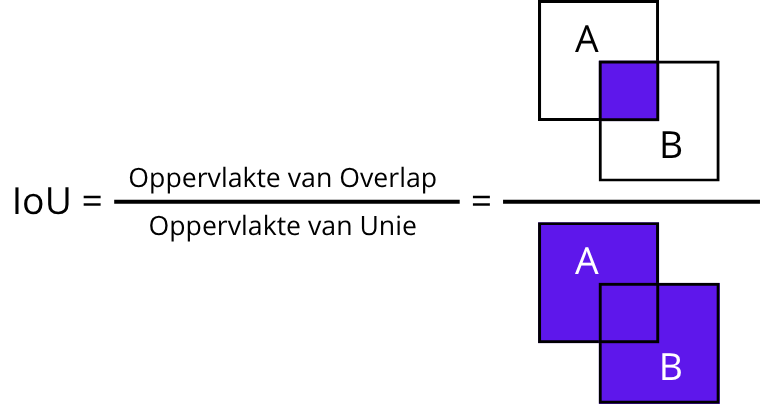
\includegraphics[width=0.6\textwidth]{iou_conceptual.png}
    \caption[Conceptuele weergave van Intersection over Union (IoU)]{
        \label{fig:iou-conceptual}
        Conceptuele weergave van Intersection over Union (IoU).
        De overlap tussen de twee rechthoeken wordt gedeeld door de unie van de twee rechthoeken.
        Dit resulteert in een waarde tussen 0 en 1, waarbij 1 betekent dat de rechthoeken volledig overlappen.
        (eigen afbeelding)
      }
\end{figure}

De matching-functie omvat de volgende conceptuele stappen:
\begin{enumerate}
    \item Voor elke frame in de vergelijkingsset worden de FastSAM-segmentaties en YOLOv11-detecties opgehaald.
    \item De objectdetectie-voorspellingen worden gefilterd op basis van de\\ \texttt{min\_pred\_conf} parameter.
    \item Indien er voor een klasse meerdere detecties zijn, wordt enkel de detectie met de hoogste vertrouwensscore behouden.
    \item Indien er geen voorspellingen overblijven na filtering, wordt de frame overgeslagen.
    \item Voor elke FastSAM-segmentatie wordt de IoU berekend met elke YOLOv11-detectie.
    \item Indien de IoU groter is dan de \texttt{iou\_threshold}, wordt de detectie beschouwd als een match voor de segmentatie.
    \item Voor elke segmentatie wordt de beste match bepaald op basis van de hoogste IoU.
    \item Tenslotte wordt de lijst van gematchte segmentaties, detecties en hun IoU-waarden opgeslagen in een dictionary per frame.
\end{enumerate}

\subsubsection{Toekennen van een Klasse aan FastSAM Object Tracks}

Ne het matchen beschikten we per frame over een lijst van FastSAM-segmentaties die 
succesvol gekoppeld konden worden aan een YOLOv11-objectdetectie.
De volgende uitdaging was om op basis van deze per-frame informatie, een definitieve klasse toe te kennen aan elk uniek FastSAM object ID
die doorheen de evaluatieopname werd gevolgd.
Een object ID kan immers over meerdere frames worden waargenomen 
en het YOLOv11-model kan in verschillende frames verschillende voorspellingen maken voor eenzelfde object (of zelfs geen voorspelling maken).
De aggregatie dient de ruis die opduikt door verschillende individuele voorspellingen, te reduceren.

Dit proces, inclusief de vorige matchingstap, werd geïmplementeerd in de overkoepelende functie \texttt{get\_predictions\_df}.
De belangrijkste conceptuele stappen zijn als volgt:

\paragraph{1. Aggregeren van Voorspellingen per FastSAM Object ID}
De eerste stap is het verzamelen van alle YOLOv11-klassevoorspellingen en hun bijbehorende 
vertrouwensscores per FastSAM object-ID, 
ongeacht in welk frame ze voorkwamen. 
Dit aggregeert de per-frame matchingresultaten naar een lijst van voorspellingen voor elke unieke getrackte entiteit.\\
De functie \texttt{get\_predictions\_per\_object\_id} voert deze groepering uit en genereert een dictionary waarin elk FastSAM object-ID is gekoppeld aan een lijst van voorspellingen.
Voor elke voorspelling wordt de klasse-ID en de bijbehorende vertrouwensscore opgeslagen.

\paragraph{2. Filteren op Minimale Observatieduur}
In de latere evaluatiestap werd ook onderzocht of het zinvol was om een parameter te introduceren die bepaalt in hoeveel frames een object moet worden waargenomen
vooraleer het wordt geclassificeerd. Dit zou eventueel een effect kunnen hebben op vals-positieve voorspellingen, omdat korte observaties meer vatbaar zijn voor ruis.
Zo worden enkel object tracks die in een minimaal aantal frames zijn waargenomen, behouden.
Dit wordt aangedreven door de parameter \texttt{min\_observed\_frames} in de functie \texttt{filter\_by\_min\_observed\_frames}.

\paragraph{3. Toekennen van de Finale Klasse per Track}
Voor elk overgebleven FastSAM object-track, werd een definitieve klasse bepaald door de functie \texttt{get\_final\_prediction\_per\_object\_id}. 
Hier werd voor elk object ID de klasse gekozen die de hoogste totale som van YOLOv11-vertrouwensscores 
behaalde over de gehele duur van de track. 
Dit kan gezien worden als een vorm van stemmingsaggregatie, 
waarbij de klasse met de meeste `stemmen' (in termen van vertrouwensscores) wordt gekozen.

\subsubsection{Samenstellen van de Finale Voorspellingsdataset}
Het resultaat van de vorige stap was een mapping van FastSAM object-ID's, 
naar hun definitieve voorspelde klasse (één van de 14 kritische objecten) 
en de geaggregeerde vertrouwensscore.
In Sectie~\ref{sec:voorbereiding-tracking-resultaten} werd al beschreven hoe de metadata van de FastSAM-trackingresultaten opgeslagen werden in zogenaamde\\ `object-datasets'.
In deze stap werden deze datasets, voor elke evaluatieopname, uitgebreid met de voorspelde klasse en de bijbehorende vertrouwensscore voor elk object ID.
Het resultaat was een finale voorspellingsdataset (pandas \texttt{Dataframe}) per evaluatieopname. Deze waren klaar was voor evaluatie en bevatten de volgende velden:
\begin{itemize}
    \item \texttt{frame\_idx}: De index van de frame in de evaluatieopname.
    \item \texttt{object\_id}: De unieke ID van het getrackte object.
    \item \texttt{gs\_confidence}: De vertrouwensscore van de FastSAM-segmentatie voor het object in de frame (dus niet van de YOLOv11-detectie).
    \item \texttt{x1, y1, x2, y2}: De coördinaten van de bounding box van de FastSAM-segmentatie in het frame.
    \item \texttt{predicted\_class\_id}: De voorspelde klasse-ID van het object, gebaseerd op de YOLOv11-detecties.
    Indien er geen voorspelling was voor het object, werd deze op -1 gezet (dit betekent dat het object als `onbekend' werd beschouwd).
    \item \texttt{predicted\_confidence}: De geaggregeerde vertrouwensscore van de voorspelde klasse, gebaseerd op de YOLOv11-detecties.
\end{itemize}

\section{Evaluatie van de Analysepipeline}

Na het implementeren van de functionaliteit voor het creëren van de finale voorspellingsdatasets, 
kon de evaluatie van de volledige analysepipeline beginnen.\\ Deze evaluatie had drie hoofddoelen:
\begin{enumerate}
    \item Het bepalen van de optimale combinatie van hyperparameterwaarden voor het eerder besproken matchingproces waarbij de finale klasse aan een track wordt toegekend.
    \item Het beoordelen van de algehele prestaties van de verschillende getrainde\\ YOLOv11-modellen tegenover de grondwaarheid op basis van precisie, recall en F1-score.
    \item Het bekomen van een kwantitatief antwoord op de deelonderzoeksvragen betreffende de accuraatheid van het 
    ontwikkelde systeem, specifiek (zoals origineel geformuleerd in Sectie~\ref{sec:onderzoeksvraag}):
        \begin{itemize}
            \item In welke mate kan de ontwikkelde software correct bepalen welke kritische objecten studenten hebben waargenomen?
            \item In welke mate kan de ontwikkelde software nauwkeurig meten hoe lang studenten naar deze objecten keken?
        \end{itemize}
\end{enumerate}

\subsection{Evaluatieprocedure}

De evaluatie van de analysepipeline werd systematisch uitgevoerd door de voorspellingsdatasets 
te vergelijken met de eerder gecreëerde grondwaarheidsdataset (zie Hoofdstuk~\ref{ch:grondwaarheid}). 
Dit proces werd net zoals de creatie van de voorspellingsdatasets,
geïmplementeerd in de notebook \texttt{13\_predict\_object\_detection.ipynb}.

\subsubsection{Definitie van de Grid Search Ruimte}

Om na te gaan welke hyperparameterwaarden het beste resultaat opleveren, werd een grid search uitgevoerd.
Een grid search is een manier om de beste combinatie van parameterwaarden te vinden door alle mogelijke combinaties uit te proberen.
Deze search werd voor de vier getrainde modellen uitgevoerd over de volgende hyperparameters:
\begin{itemize}
    \item \textbf{training\_sample\_count}: Een impliciete parameter die het aantal trainingssamples per klasse bepaalt, die gebruikt werden voor het trainen van de modellen.
    \item \textbf{min\_pred\_conf}: De minimum vereiste vertrouwensscore voor een YOLOv11-detectie om als geldig te worden beschouwd.
    \item \textbf{iou\_threshold}: De minimum Intersection over Union (IoU) drempel die vereist is om een match tussen een FastSAM-segmentatie en een YOLOv11-detectie te beschouwen als geldig.
    \item \textbf{min\_observed\_frames}: Het minimum aantal frames waarin een object moet worden waargenomen alvorens het wordt geclassificeerd.
\end{itemize}
Zie Codefragment~\ref{listing:grid-search} voor de gebruikte waarden voor deze hyperparameters, 
inclusief de overkoepelende logica voor het opstellen van het resultaat van de grid search.

\begin{listing}[H]
  \begin{minted}{python}
ground_truth_df = experiment_utils.get_ground_truth_df(IGNORED_CLASS_IDS)

min_pred_confs = [0.5, 0.55, 0.6, 0.65, 0.7, 0.75, 0.8, 0.85, 0.9]
iou_thresholds = [0.05, 0.1, 0.2, 0.3, 0.4, 0.5, 0.6]
min_observed_frames = [0, 1, 3, 5, 7]

grid_search_params = list(
    itertools.product(min_pred_confs, iou_thresholds, min_observed_frames)
)

grid_search_results = []
for i, model_path in enumerate(models):
    print(f"Evaluating model {i + 1}/{len(models)}: {model_path.stem}")

    model = YOLO(model_path)
    model_grid_search_results = evaluate_model(
        model_name=model_path.stem,
        model_class_names=model.names,
        ground_truth_df=ground_truth_df,
        grid_search_params=grid_search_params,
    )
    grid_search_results.extend(model_grid_search_results)
  \end{minted}
  \caption[Code voor het uitvoeren van de grid search over hyperparameters]{
    \label{listing:grid-search}
        De code voor het uitvoeren van de grid search over de hyperparameters.
        Eerst wordt de grondwaarheid geladen en worden de hyperparameterwaarden gedefinieerd. 
        Vervolgens wordt voor elk model de evaluatiefunctie \texttt{evaluate\_model} aangeroepen.
        Deze functie evalueert de prestaties van het model over alle combinaties van hyperparameters.
        De resultaten van de grid search worden opgeslagen in een lijst.
    }
\end{listing}

\subsubsection{Evaluatie van de Modellen}

Voor elk model wordt de overkoepelende functie \texttt{evaluate\_model} aangeroepen,
die elke mogelijke combinatie van hyperparameters evalueert.
Belangrijk om op te merken is dat, hoewel we hier de verschillende getrainde YOLOv11-modellen evalueren,
we op hetzelfde moment dit ook doen voor de gehele pipeline, inclusief de FastSAM-tracking.
Aangezien er in totaal 315 mogelijke combinaties zijn, 
maakt deze functie gebruik van \texttt{multiprocessing} om de evaluatie van de modellen te versnellen.
Het stuurt elke combinatie van hyperparameters naar een apart subproces,
uitgevoerd door de functie \texttt{evaluate\_grid\_combination} (zie Codefragment~\ref{listing:evaluate-grid-combination}).

\begin{listing}[H]
  \fontsize{10pt}{10pt}
  \begin{minted}{python}
    def evaluate_grid_combination(
        model_name: str,
        model_class_names: dict[int, str],
        ground_truth_df: pd.DataFrame,
        min_pred_conf: float,
        iou_threshold: float,
        min_observed_frames: int,
    ):
        # Lege confusion matrix aanmaken
        cm = experiment_utils.create_confusion_matrix(IGNORED_CLASS_IDS)
        
        # Lege evaluatie DataFrame aanmaken
        full_evaluation_df = pd.DataFrame()

        comparison_sets = (COMPARISON_SETS_PATH / model_name).iterdir()
        for comparison_set_path in comparison_sets:
            recording_id = comparison_set_path.stem

            # Voor elke evaluatieopname, de voorspellingen berekenen
            predictions_df = get_predictions_df(
                model_class_names=model_class_names,
                comparison_set_path=comparison_set_path,
                min_pred_conf=min_pred_conf,
                iou_threshold=iou_threshold,
                min_observed_frames=min_observed_frames,
            )

            # De grondwaarheid voor de huidige opname ophalen
            gt_df_recording = ground_truth_df[ground_truth_df["recording_id"] == recording_id]

            # Evalueren van de voorspellingen
            eval_df = experiment_utils.evaluate_predictions(
                predictions_df=predictions_df,
                gt_df=gt_df_recording,
            )

            # Voorspellingsresultaten toevoegen aan de volledige evaluatie DataFrame
            full_evaluation_df = pd.concat(
                [full_evaluation_df, eval_df.assign(recording_id=recording_id)],
                ignore_index=True,
            )

            # Confusion matrix bijwerken met de evaluatieresultaten
            experiment_utils.update_confusion_matrix(cm, eval_df)

        # Metrieken van de confusion matrix berekenen (precision, recall, F1-score, etc.)
        cm_metrics = experiment_utils.confusion_matrix_metrics(cm)

        # Valideren van de confusion matrix
        validate_confusion_matrix(cm_metrics, ground_truth_df)

        return full_evaluation_df, cm, cm_metrics
  \end{minted}
  \caption[Functie voor het evalueren van een enkele combinatie van hyperparameters]{
      \label{listing:evaluate-grid-combination}
      De \texttt{evaluate\_grid\_combination} functie evalueert een enkele combinatie van hyperparameters voor een model over de volledige collectie van evaluatieopnames.
      Het laadt de grondwaarheid en de voorspellingsdataset en berekent de evaluatiemetrieken.
      De functie retourneert een DataFrame met de evaluatieresultaten, de confusion matrix en zijn metrieken.
    }
\end{listing}

De \texttt{evaluate\_grid\_combination} functie berekent drie belangrijke outputs:
\begin{itemize}
    \item \textbf{full\_evaluation\_df}: Een DataFrame met de evaluatieresultaten voor elk frame van elke evaluatieopname.
    Dit bevat informatie zoals de voorspelde klasse, de grondwaarheidsklasse en de bijbehorende metriekwaarden.
    \item \textbf{cm}: De confusion matrix die de prestaties van het model over alle evaluatieopnames heen samenvat.
    Deze matrix toont het aantal correcte en onjuiste voorspellingen per klasse.
    \item \textbf{cm\_metrics}: Berekende metriekwaarden (precisie, recall, F1-score, etc.) op basis van de confusion matrix.
\end{itemize}

Het creëren van deze drie outputs gebeurt in de volgende stappen:

\paragraph{1. Creatie van de Evaluatie DataFrame}
De evaluatiedataframe wordt berekend door de functie\\ \texttt{experiment\_utils.evaluate\_predictions},
die de voorspellingen vergelijkt met de grondwaarheid voor elke frame van de evaluatieopname.
Het voegt voor elke frame twee zaken toe aan de voorspellingsdataset:
\begin{itemize}
    \item \textbf{true\_class\_id}: De klasse-ID van het object zoals gedefinieerd in de grondwaarheid.
    \item \textbf{label}: Een categorisch label dat aangeeft hoe de voorspelling zich verhoudt tot die grondwaarheid. Dit label kan de volgende waarden aannemen:
        \begin{itemize}
            \item \textbf{TP (True Positive)}: De voorspelde klasse komt overeen met de grondwaarde klasse voor een object in hetzelfde frame. 
            Een correcte detectie en classificatie.
            \item \textbf{FP (False Positive):} Het model voorspelt een object, maar er is geen overeenkomstige grondwaarheid 
            voor die klasse in het frame; of het voorspelde object komt niet overeen met de grondwaarheidsklasse.
            \item \textbf{TN (True Negative):} Het model voorspelt correct dat er geen object bekeken werd (voorspelt -1, of `onbekend') 
            en er is inderdaad geen overeenkomstige grondwaarheid binnen dit frame.
            \item \textbf{FN (False Negative):} Er is een object in de grondwaarheid aanwezig, maar het model heeft dit object niet gedetecteerd of geclassificeerd.
        \end{itemize} 
\end{itemize}
Ook werd het veld \texttt{mask\_area} vervangen door zijn waarde in de \texttt{grondwaarheid}, om latere analyses mogelijk te maken.
Indien het ging om een vals-positief waar geen grondwaarheid voor bestond, werd hier een lege waarde (\texttt{NaN}) toegekend. 

Hier is het interessant om stil te staan bij twee specifieke gevallen:
Wanneer de evaluatie een vals-positief aangeeft waarvoor geen grondwaarheid bestaat, werd hier een speciale klasse-ID -3 toegekend als `ware klasse' (met als naam `geen grondwaarheid').
Wanneer de evaluatie een vals-negatief aangeeft, werd de klasse-ID -2 toegekend als `voorspelde klasse' (met als naam `geen voorspelling').
Dit maakte het mogelijk om deze gevallen mee te visualiseren in de confusion matrix.

\paragraph{2. Bijwerken van de Confusion Matrix}
De confusion matrix is een vierkante tabel die het mogelijk maakt om de prestaties van het model te visualiseren en metrieken zoals precisie, recall en F1-score te berekenen.
De matrix bestaat uit rijen en kolommen die overeenkomen met de verschillende klassen.
Elke rij vertegenwoordigt de ware klasse (grondwaarheid), terwijl elke kolom de voorspelde klasse voorstelt.\\
De functie \texttt{experiment\_utils.update\_confusion\_matrix} wordt gebruikt om de confusion matrix bij 
te werken op basis van de evaluatieresultaten voor een bepaalde evaluatieopname (zie Codefragment~\ref{listing:update-confusion-matrix}).

\begin{listing}[H]
  \begin{minted}{python}
    def update_confusion_matrix(
        confusion_mat: pd.DataFrame, eval_df: pd.DataFrame
    ) -> pd.DataFrame:
        for _, row in eval_df.iterrows():
            true = row.get("true_class_id")
            pred = row.get("predicted_class_id")

            if pd.isna(true): # Als er geen grondwaarheid is
                if pred == UNKNOWN_CLASS_ID:
                    # Dit is een waar-negatief (TN), 
                    # en wordt niet meegeteld in de confusion matrix.
                    continue

                # Dit is een vals-positief (FP) voor de voorspelde klasse.
                true = MISSING_GROUND_TRUTH_CLASS_ID

            t = int(true)
            p = int(pred)
            if t in confusion_mat.index and p in confusion_mat.columns:
                confusion_mat.loc[t, p] += 1
  \end{minted}
  \caption[Functie voor het bijwerken van de confusion matrix]{
      \label{listing:update-confusion-matrix}
        De \texttt{update\_confusion\_matrix} functie werkt de confusion matrix bij op basis van de evaluatieresultaten.
        Voor elke rij in het evaluatiedataframe wordt het aantal voorspellingen in de cel met de ware klasse en de voorspelde klasse verhoogd.
        Indien er geen grondwaarheid is, en het model toch een klasse voorspelt, wordt dit beschouwd als een vals-positief (FP).
      }
\end{listing}

\paragraph{3. Berekekenen van Confusion Matrix Metrieken}
Uit de confusion matrix kunnen verschillende metrieken worden afgeleid die de prestaties van het model samenvatten.
Dit gebeurt met behulp van de functie \texttt{experiment\_utils.confusion\_matrix\_metrics}. 

Voor elke individuele objectklasse (met uitzondering van de speciale klassen voor FP/FN) worden de volgende metrieken berekend:
\begin{itemize}
    \item \textbf{Precisie (Precision)}: Deze metriek meet het aandeel van de correct voorspel\-de instanties (True Positives, TP) 
        ten opzichte van alle voorspelde instanties binnen die klasse (TP + False Positives, FP). 
        Een hoge precisie betekent dat wanneer het model een bepaalde klasse toekent aan een object, die voorspelling meestal correct is. 
        Met andere woorden, het geeft een indicatie over hoeveel vals-positieven het model maakt. 
        Optimalisatie van precisie kan echter leiden tot een afname van recall,
        omdat het model mogelijk minder objecten van die klasse detecteert om vals-positieven te vermijden.
        \[
        \text{Precisie}_{\text{klasse}} = \frac{\text{TP}_{\text{klasse}}}{\text{TP}_{\text{klasse}} + \text{FP}_{\text{klasse}}}
        \]
    \item \textbf{Recall}: Dit meet het aandeel van de correct voorspelde instanties (TP) 
        van een klasse ten opzichte van alle daadwerkelijke instanties in de grondwaarheid (TP + False Negatives, FN). 
        Het geeft aan hoe goed het model in staat is om alle relevante objecten van een bepaalde klasse te herkennen.
        Een hoge recall betekent dat het model weinig vals-negatieven geeft.
        Overoptimalisatie van recall kan echter leiden tot een toename van vals-positieven.
        \[
        \text{Recall}_{\text{klasse}} = \frac{\text{TP}_{\text{klasse}}}{\text{TP}_{\text{klasse}} + \text{FN}_{\text{klasse}}}
        \]
    \item \textbf{F1-score}: Het harmonisch gemiddelde van precisie en recall voor een klasse, 
    die een gebalanceerde maatstaf biedt door zowel de precisie als de recall in overweging te nemen.
    \[
    \text{F1-score}_{\text{klasse}} = 2 \times \frac{\text{Precisie}_{\text{klasse}} \times \text{Recall}_{\text{klasse}}}{\text{Precisie}_{\text{klasse}} + \text{Recall}_{\text{klasse}}}
    \]
    \item \textbf{Support}: Het aantal daadwerkelijke instanties van een klasse in de grondwaarheidsdataset (de som van een rij in de confusion matrix voor die klasse).
\end{itemize}

Naast deze per-klasse metrieken worden ook \textbf{micro-gemiddelde} precisie, recall en F1-score berekend. 
Bij micro-averaging worden eerst de globale totalen van True Positives, False Positives, en False Negatives over alle klassen heen gesommeerd. 
Vervolgens worden de metrieken op basis van deze globale totalen berekend (net zoals hierboven beschreven, maar dan met de micro-totalen).
Dit geeft een algemeen overzicht van de prestaties van het model over alle klassen heen.

\subsection{Resultaten van de Hyperparameter Grid Search}

Op basis van F1-score werd voor elk model de beste combinatie van hyperparameters bepaald.
De precisie, recall en F1-score voor het beste resultaat per model worden weergegeven in Figuur~\ref{fig:best-models-metrics}.
\begin{figure}[H]
  \centering
  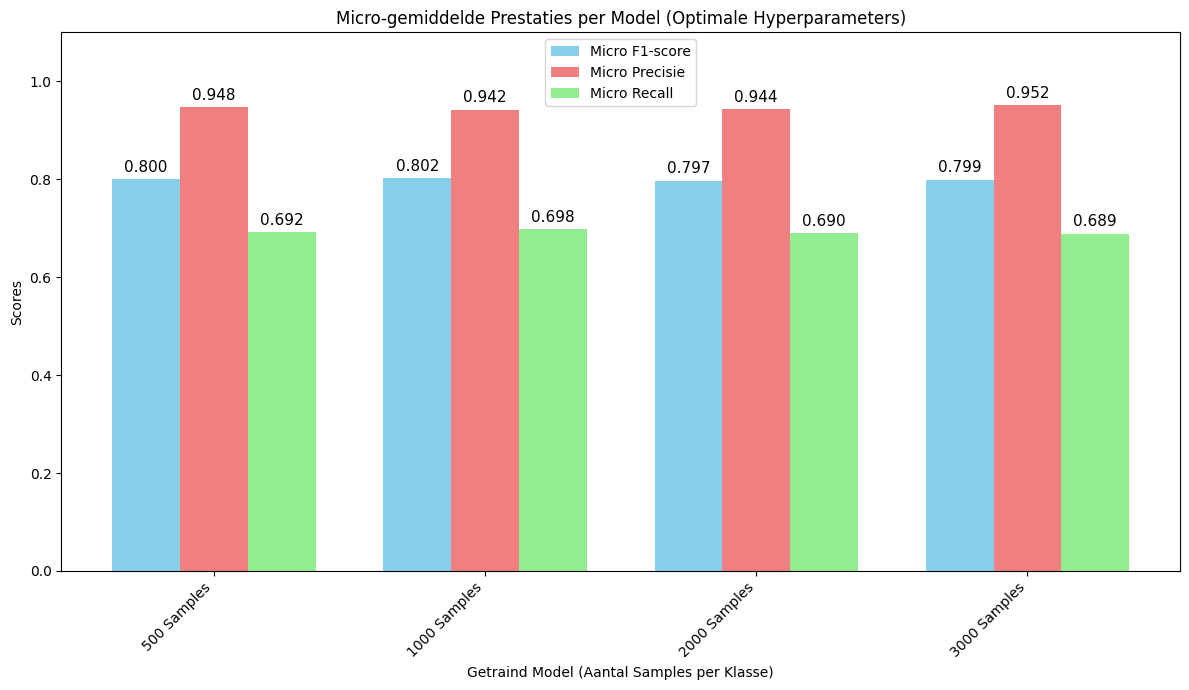
\includegraphics[width=1\textwidth]{grid-search-results-models.png}
  \caption[]{\label{fig:best-models-metrics} 
    De precisie, recall en F1-score van de beste modellen per getraind YOLOv11-model.
    De beste hyperparameters werden bepaald op basis van de hoogste F1-score over alle evaluatieopnames.
    De resultaten zijn weergegeven voor de vier getrainde modellen, gesorteerd op de hoeveelheid samples die gebruikt werden voor het trainen.
    }
\end{figure}
Merk op dat de resultaten van elk model hier heel nauw bij elkaar liggen, wat misschien onverwacht lijkt.
Dit wijst echter potentieel op het feit dat de beperkende factor in de prestaties van de analysepipeline niet de YOLOv11-objectdetectie is,
maar eerder de FastSAM-tracking en segmentatie stap.

Volgens de grid search werd het beste model getraind op 1000 samples per klasse, die de volgende resultaten behaalde:
\begin{itemize}
    \item \textbf{Precisie:} 0.9424
    \item \textbf{Recall:} 0.6976
    \item \textbf{F1-score:} 0.8017
\end{itemize}
De beste combinatie van hyperparameters voor dit model zijn:
\begin{itemize}
    \item \textbf{min\_pred\_conf:} 0.85
    \item \textbf{iou\_threshold:} 0.2
    \item \textbf{min\_observed\_frames:} 3
\end{itemize}
De confusion matrix voor dit model is weergegeven in Figuur~\ref{fig:confusion-matrix-best-model}.
We zien dat er binnen de objecten in de grondwaarheid geen enkele vals-positief te bespeuren valt.
We zien echter wel dat er een aantal vals-positieven zonder grondwaarheid zijn (de rij `geen grondwaarheid' in de matrix).
Een hypothese is dat een groot deel van deze zogezegde vals-positieven eigenlijk objecten zijn die correct gedetecteerd zijn, 
maar die niet in de grondwaarheidsdataset werden opgenomen.
Dit wordt in een latere sectie verder onderzocht.

\begin{figure}[H]
  \centering
  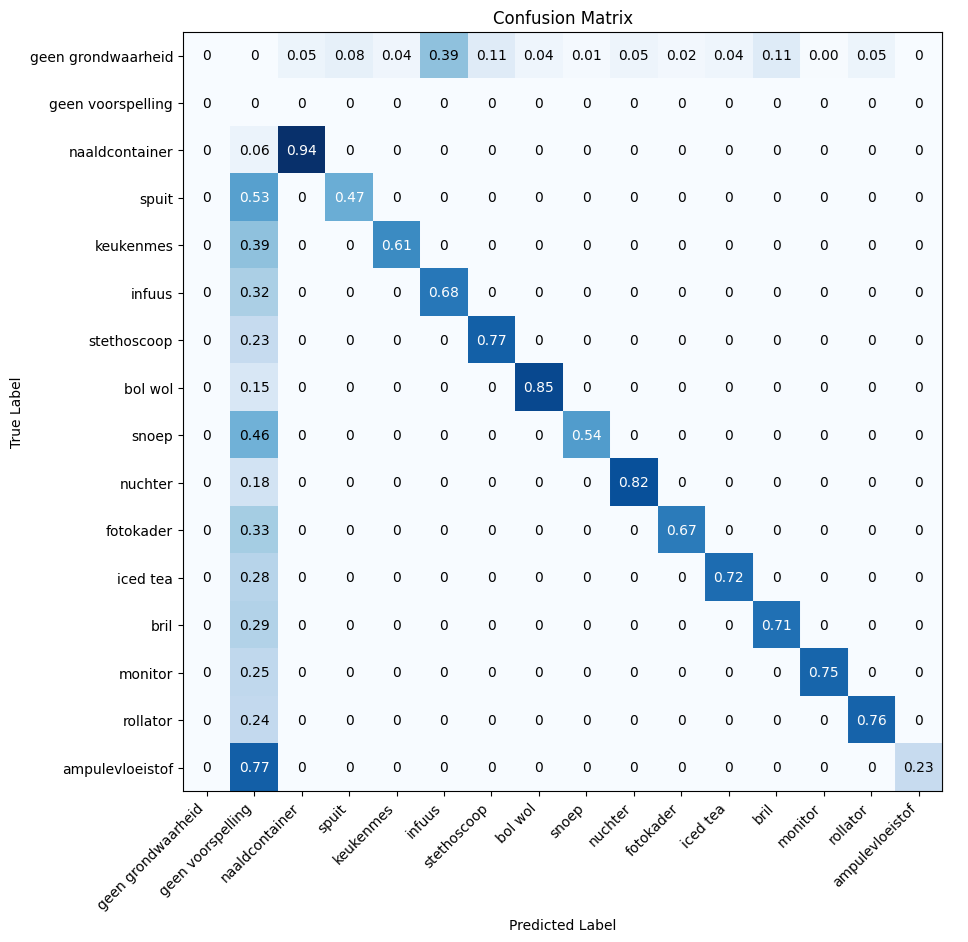
\includegraphics[width=1\textwidth]{confusion-matrix-best-model.png}
  \caption[]{\label{fig:confusion-matrix-best-model} 
    De confusion matrix voor het beste model, getraind op 1000 samples per klasse.
    Hier zijn de totaalwaarden van elke cel genormaliseerd door te delen door de som van de waarden in zijn rij.
    Elke rij in de matrix vertegenwoordigt de ware klasse (grondwaarheid),
    terwijl elke kolom staat voor de voorspelde klasse.
    Merk op dat er twee specifieke klassen zijn toegevoegd, namelijk `geen grondwaarheid' 
    wat wijst op vals-positieven en `geen voorspelling' wat wijst op vals-negatieven.
    De diagonaal van de matrix toont de correcte voorspellingen,
    terwijl de andere cellen de fouten van het model weergeven.
  }
\end{figure}

\subsection{Verdere Analyse van het Beste Model}

Om een beter inzicht te krijgen in de prestaties van de analysepipeline en om mogelijk problemen te identificeren, werden de 
resultaten van het beste model (getraind op 1000 samples per klasse) verder geanalyseerd.

\subsubsection{Analyse van de Vals-Positieven}

Eerst werden de vals-positieven per klasse geanalyseerd door middel van een staafdiagram 
om een algemeen overzicht te krijgen van de verdeling van vals-positieven over de verschillende objectklassen (zie Figuur~\ref{fig:false-positives-per-class}).
De aantallen werden genormaliseerd ten opzichte van de support van die klasse om een eerlijke vergelijking te verkrijgen.
Opmerkelijk is dat het `infuus' object veruit de meeste vals-positieven geeft, wat wijst op een meer systematisch probleem met de detectie van dit object.

\begin{figure}[H]
  \centering
  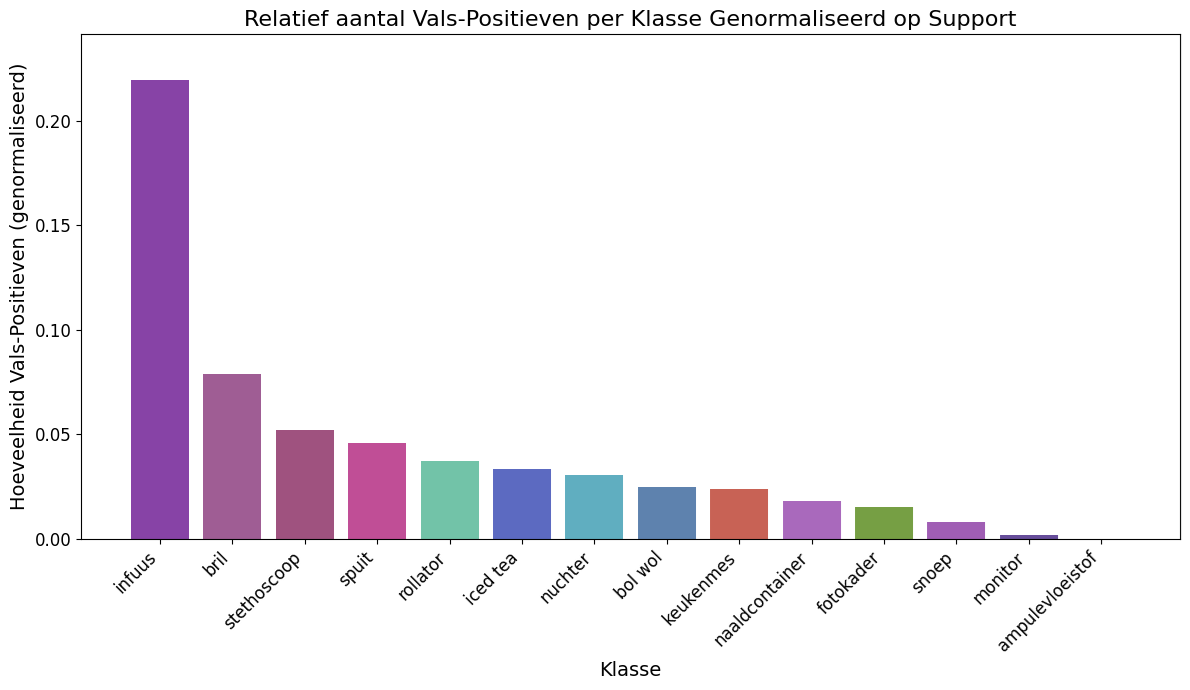
\includegraphics[width=1\textwidth]{false-positives-per-class.png}
  \caption[]{\label{fig:false-positives-per-class}
    Staafdiagram van het aantal vals-positieven per klasse voor het beste model, genormaliseerd ten opzichte van de support van die klasse.

  }
\end{figure}

Om verder inzicht te verkrijgen in de aard van de vals-positieven, werden per klasse de uitsnedes van elk vals-positief object manueel bekeken.
Hier is het belangrijk om te vermelden dat de uitsnedes betrekking hebben op de FastSAM-segmenta\-ties,
en niet op de YOLOv11-detecties.
Voor voorbeelden van deze uitsnedes binnen de klasse `naaldcontainer', zie Figuur~\ref{fig:fp-examples-naaldcontainer}.
Zoals men kan zien, zijn alle vals-positieven in de werkelijkheid toch correcte detecties, maar werden ze niet opgenomen in de grondwaarheid dataset.
Een mogelijke verklaring hiervoor is dat de segmentatiemaskers van de FastSAM-tracking niet altijd volledig 
overeenkomen met de grondwaarheid.
Dit zorgt ervoor dat sommige objecten als `bekeken' aangeduid worden in de geautomatiseerde analyse, 
terwijl ze niet opgenomen werden in de grondwaarheid omdat er geen overlap was met het blikpunt van de student.
\begin{figure}[H]
    \centering
    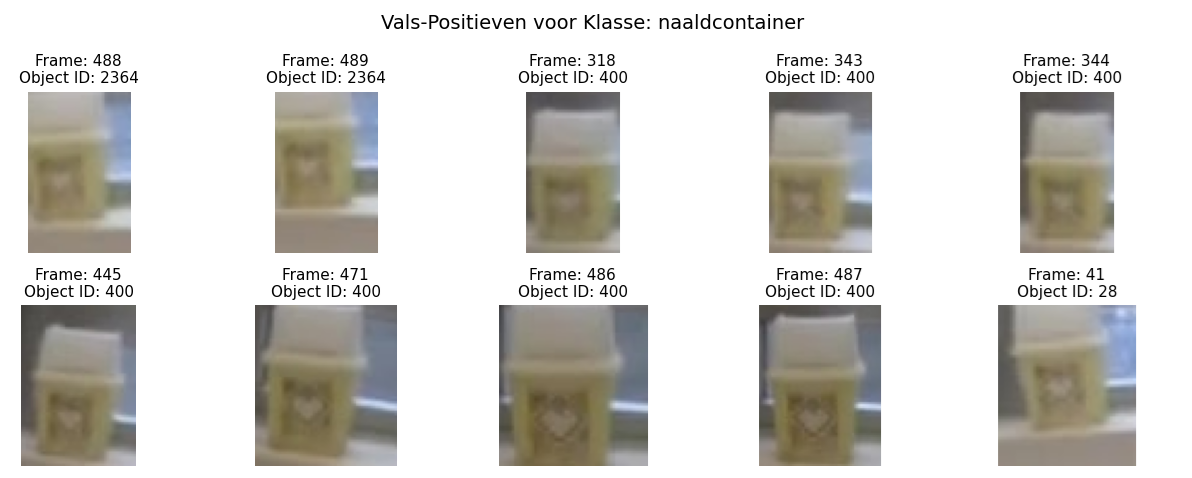
\includegraphics[width=1\textwidth]{fp-examples-naaldcontainer.png}
    \caption[]{\label{fig:fp-examples-naaldcontainer}
    Vals-positieve voorbeelden voor de klasse `naaldcontainer' van het beste model.
    De afbeeldingen tonen de uitsnedes van de FastSAM-segmentaties die als vals-positief werden beschouwd, vergeleken met de grondwaarheid.
    Het framenummer en de klasse-ID van de FastSAM-segmentatie zijn weergegeven in de titel van elke afbeelding.
    }
\end{figure}

Voor elke klasse werden op deze manier de uitsnedes van de vals-positieven manueel bekeken om te bepalen of ze in werkelijkheid ook vals-positief waren.
Uit het totaal van 262 zogezegde vals-positieven, bleken er echter slechts drie `echte' vals-positieven te zijn (met uitzondering van het infuus is, dat hierna wordt besproken).
Interessant was dat deze drie vals-positieven allemaal betrekking hadden op de klasse `fotokader', en ook tot dezelfde FastSAM object ID behoorden (zie Figuur~\ref{fig:fp-examples-fotokader}).
Dit wijst op een fout in de tracking van dit specifieke object, veroorzaakt door het onjuist toekennen van een object ID aan een segmentatie die niet tot hetzelfde object behoort.
Inderdaad, bij manuele inspectie van de resultaten bleek dat de meeste frames met dit object ID eigenlijk betrekking hadden tot het effectief bekeken fotokader.
Echter, wanneer de student het hoofd draaide, bleef de FastSAM-tracking andere objecten toewijzen aan dit object ID, waardoor vals-positieven ontstonden.
Dit kan eventueel worden opgelost in de toekomst na een meer uitgebreide analyse van dit probleem in de FastSAM-tracking.

\begin{figure}[H]
  \centering
  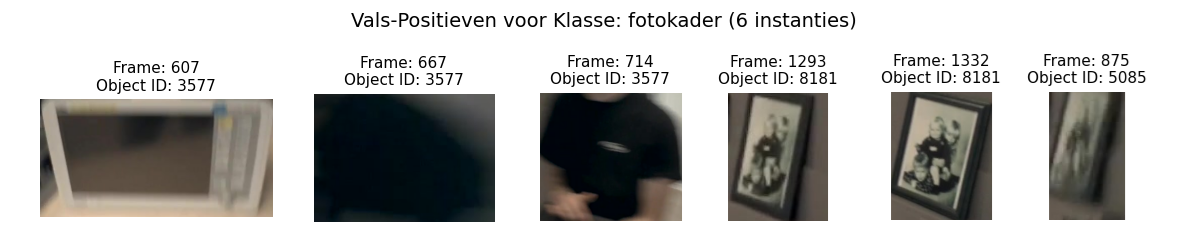
\includegraphics[width=1\textwidth]{fp-fotokader.png}
  \caption[]{\label{fig:fp-examples-fotokader}
    Vals-positieve voorbeelden voor de klasse `fotokader' van het beste model.
    Hier zien we drie `ware' vals-positieven, en drie vals-positieven die in werkelijkheid correcte detecties waren. 
    }
\end{figure}

Bij de vals-positieven verdient het infuus een aparte vermelding.
Het model heeft in totaal 102 vals-positieven voorspeld voor deze klasse.
In Figuur~\ref{fig:fp-infuus} zien we enkele willekeurige uitsnedes van deze vals-positieven.
Echter, bij manuele inspectie bleken de uitsnedes van deze voorspellingen toch het infuus te bevatten.
De definitie van `vals-positief' steunt bij dit object op de definitie van wat begrepen wordt onder `bekeken'.
In de grondwaarheid werden enkel de zak en de druppelteller van het infuus opgenomen;
terwijl de analyse ook het infuus detecteert wanneer de student enkel naar de infuuspaal kijkt.
Als men enkel wil weten of de student naar de infuuszak of druppelteller kijkt, dan zijn dit inderdaad vals-positieven.
De waarneming valt te verklaren door het feit dat FastSAM het volledige infuus, inclusief de paal en de voet, detecteert.
Vervolgens detecteert het YOLOv11-model de infuuszak en de druppelteller, waarvan de bounding-box overlapt met de FastSAM-segmentatie.
Bij een lage minimum vereiste IoU drempel, worden deze segmentaties dus ook geclassificeerd als `infuus'.
Deze bevinding wijst op problemen bij de detectie van objecten die samengesteld zijn uit meerdere componenten.

\begin{figure}[H]
  \centering
  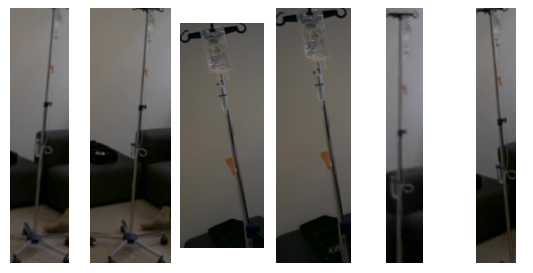
\includegraphics[width=1\textwidth]{fp-infuus.png}
  \caption[]{\label{fig:fp-infuus}
    Vals-positieve voorbeelden voor de klasse `infuus' van het beste model.
    }
\end{figure}

\subsubsection{Analyse van de Vals-Negatieven}

Om het effect van het type object op de prestaties van het model te onderzoeken,
werden vals-negatieven per klasse (van het beste model) geanalyseerd (zie Figuur~\ref{fig:fn-per-class}).
De aantallen werden opnieuw genormaliseerd ten opzichte van de support van die klasse om een eerlijke vergelijking te verkrijgen.
Uit deze analyse bleken de klassen `ampule vloeistof', `spuit' en `snoep', de meeste vals-negatieven op te leveren.
Dit is logisch, aangezien deze objecten klein zijn, waardoor ze moeilijk te detecteren bleken.
De `ampule vloeistof' en de `spuit' waren heel doorschijnend, met een witte achtergrond.
Hoewel het snoepje heel klein was, werden toch meer dan 50\% van de gevallen correct gedetecteerd. 

\begin{figure}[H]
  \centering
  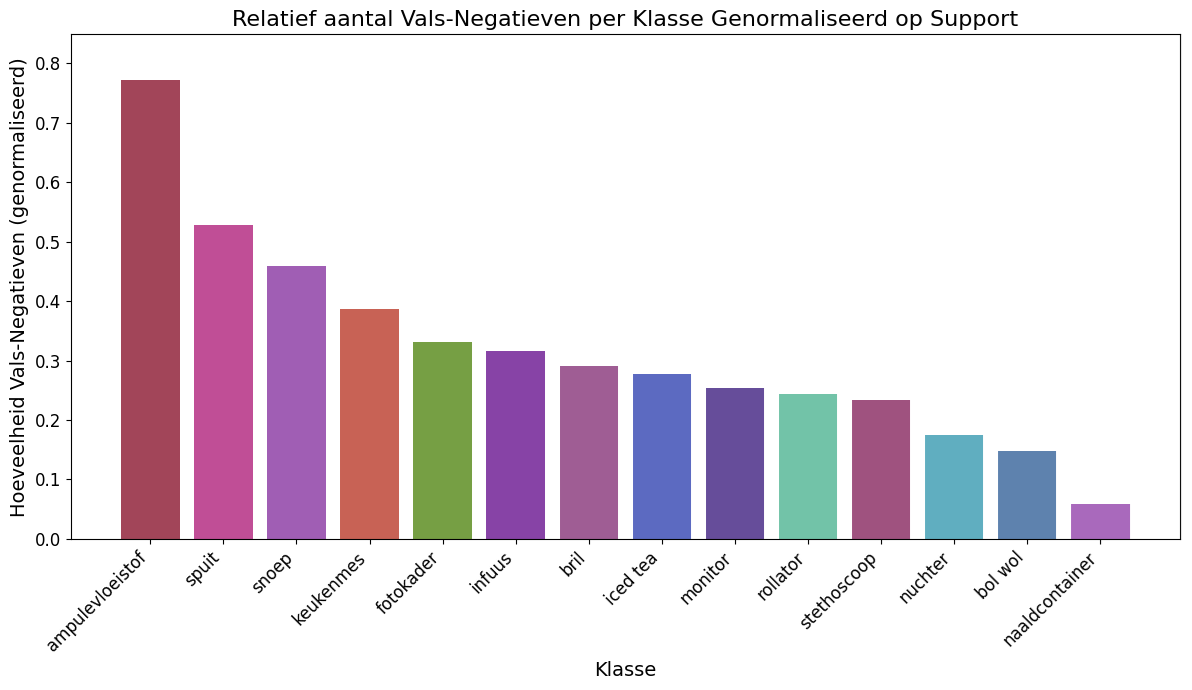
\includegraphics[width=1\textwidth]{fn-per-class.png}
  \caption[]{\label{fig:fn-per-class}
    Staafdiagram van het aantal vals-negatieven per klasse voor het beste model, genormaliseerd ten opzichte van de support van die klasse.
  }
\end{figure}

Het verwerven van een beter inzicht in de aard van de vals-negatieven vereiste echter een meer diepgaande analyse.

\paragraph{Analyse van de Maskergroottes van Vals-Negatieven en Waar-Positieven}
Als hypothese kunnen we stellen dat de analysepipeline vooral kleine objecten mist. 
Om dit te onderzoeken, werden de maskergroottes van de waar-positieven (TP) en vals-negatieven (FN) per klasse geanalyseerd.
Voor elke klasse werd `\text{Cohen's d}' berekend, een maatstaf voor de effectgrootte die aangeeft hoe groot het verschil is tussen de gemiddelde maskergrootte van de TP en FN (zie Figuur~\ref{fig:cohens-d-fn-tp}).
% TODO: formule voor Cohen's d toevoegen? also, kan deze zin beter, also cohens d in aanhalingstekens
Boven elke staaf in de figuur staat ook het gehalte aan vals-negatieven voor die klasse, tegenover de support ervan.
Dit geeft een indicatie over de betrouwbaarheid van de effectgrootte, aangezien een hoge effectgrootte bij een laag aantal vals-negatieven mogelijk niet representatief is.
We zien dat de meeste klassen een gemiddelde tot hoge effectgrootte tonen, wat betekent dat de TP gemiddeld grotere maskers bevat dan de FN.

\begin{figure}[H]
  \centering
  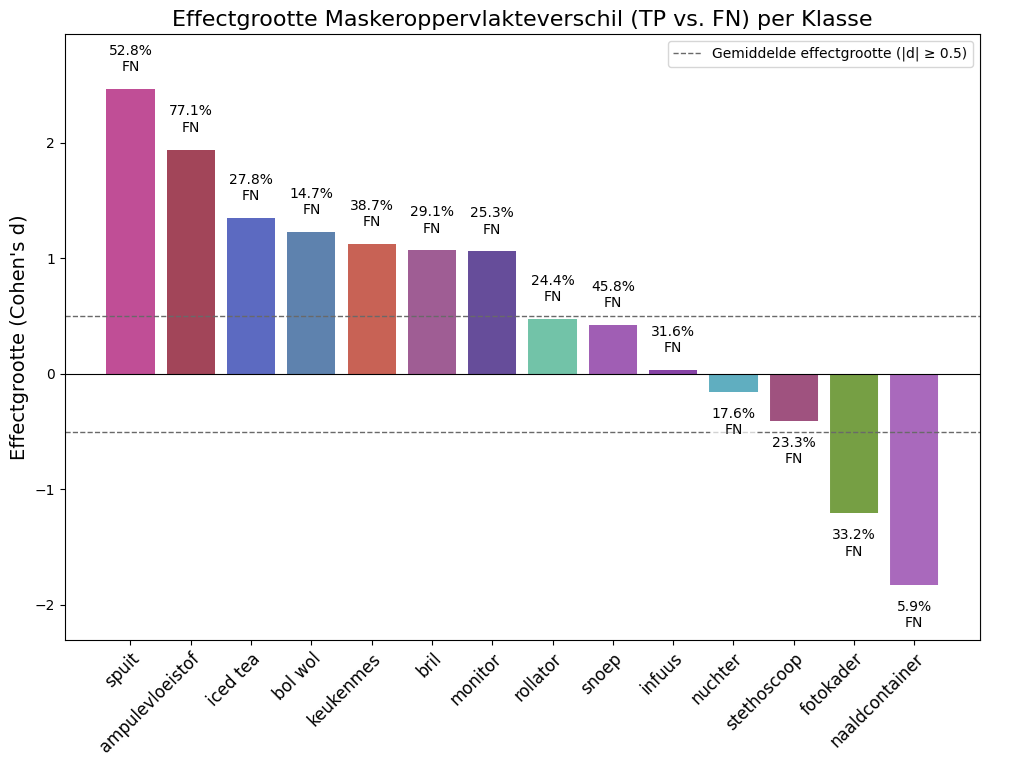
\includegraphics[width=1\textwidth]{cohens-d-tp-fn.png}
  \caption[]{\label{fig:cohens-d-fn-tp}
    Cohen's d voor de gemiddelde maskergrootte van de waar-positieven (TP) en vals-negatieven (FN) per klasse.
    Boven elke staaf staat het percentage vals-negatieven ten opzichte van de support van die klasse.
    Een positieve waarde duidt erop dat de TP gemiddeld grotere maskers bevat dan de FN, terwijl een negatieve waarde het omgekeerde aangeeft.
    Een waarde van 0.2 wordt vaak beschouwd als een klein effect, 0.5 als een gemiddeld effect, en 0.8 als een groot effect.
  }
\end{figure}

Om een beter inzicht te krijgen in de distributie van de maskergroottes binnen zowel de TP als de FN, werden voor elke klasse vioolplotten gemaakt (zie Figuur~\ref{fig:violinplot-fn-tp}).
Deze plots tonen de verdeling van de maskergroottes voor zowel de TP als de FN, waarbij de breedte van elke viool de dichtheid van de waarden aangeeft.
Hier zijn de klassen van links naar rechts en van boven naar beneden geordend volgens hun `\text{Cohen's d}' waarde.

\begin{figure}[H]
  \centering
  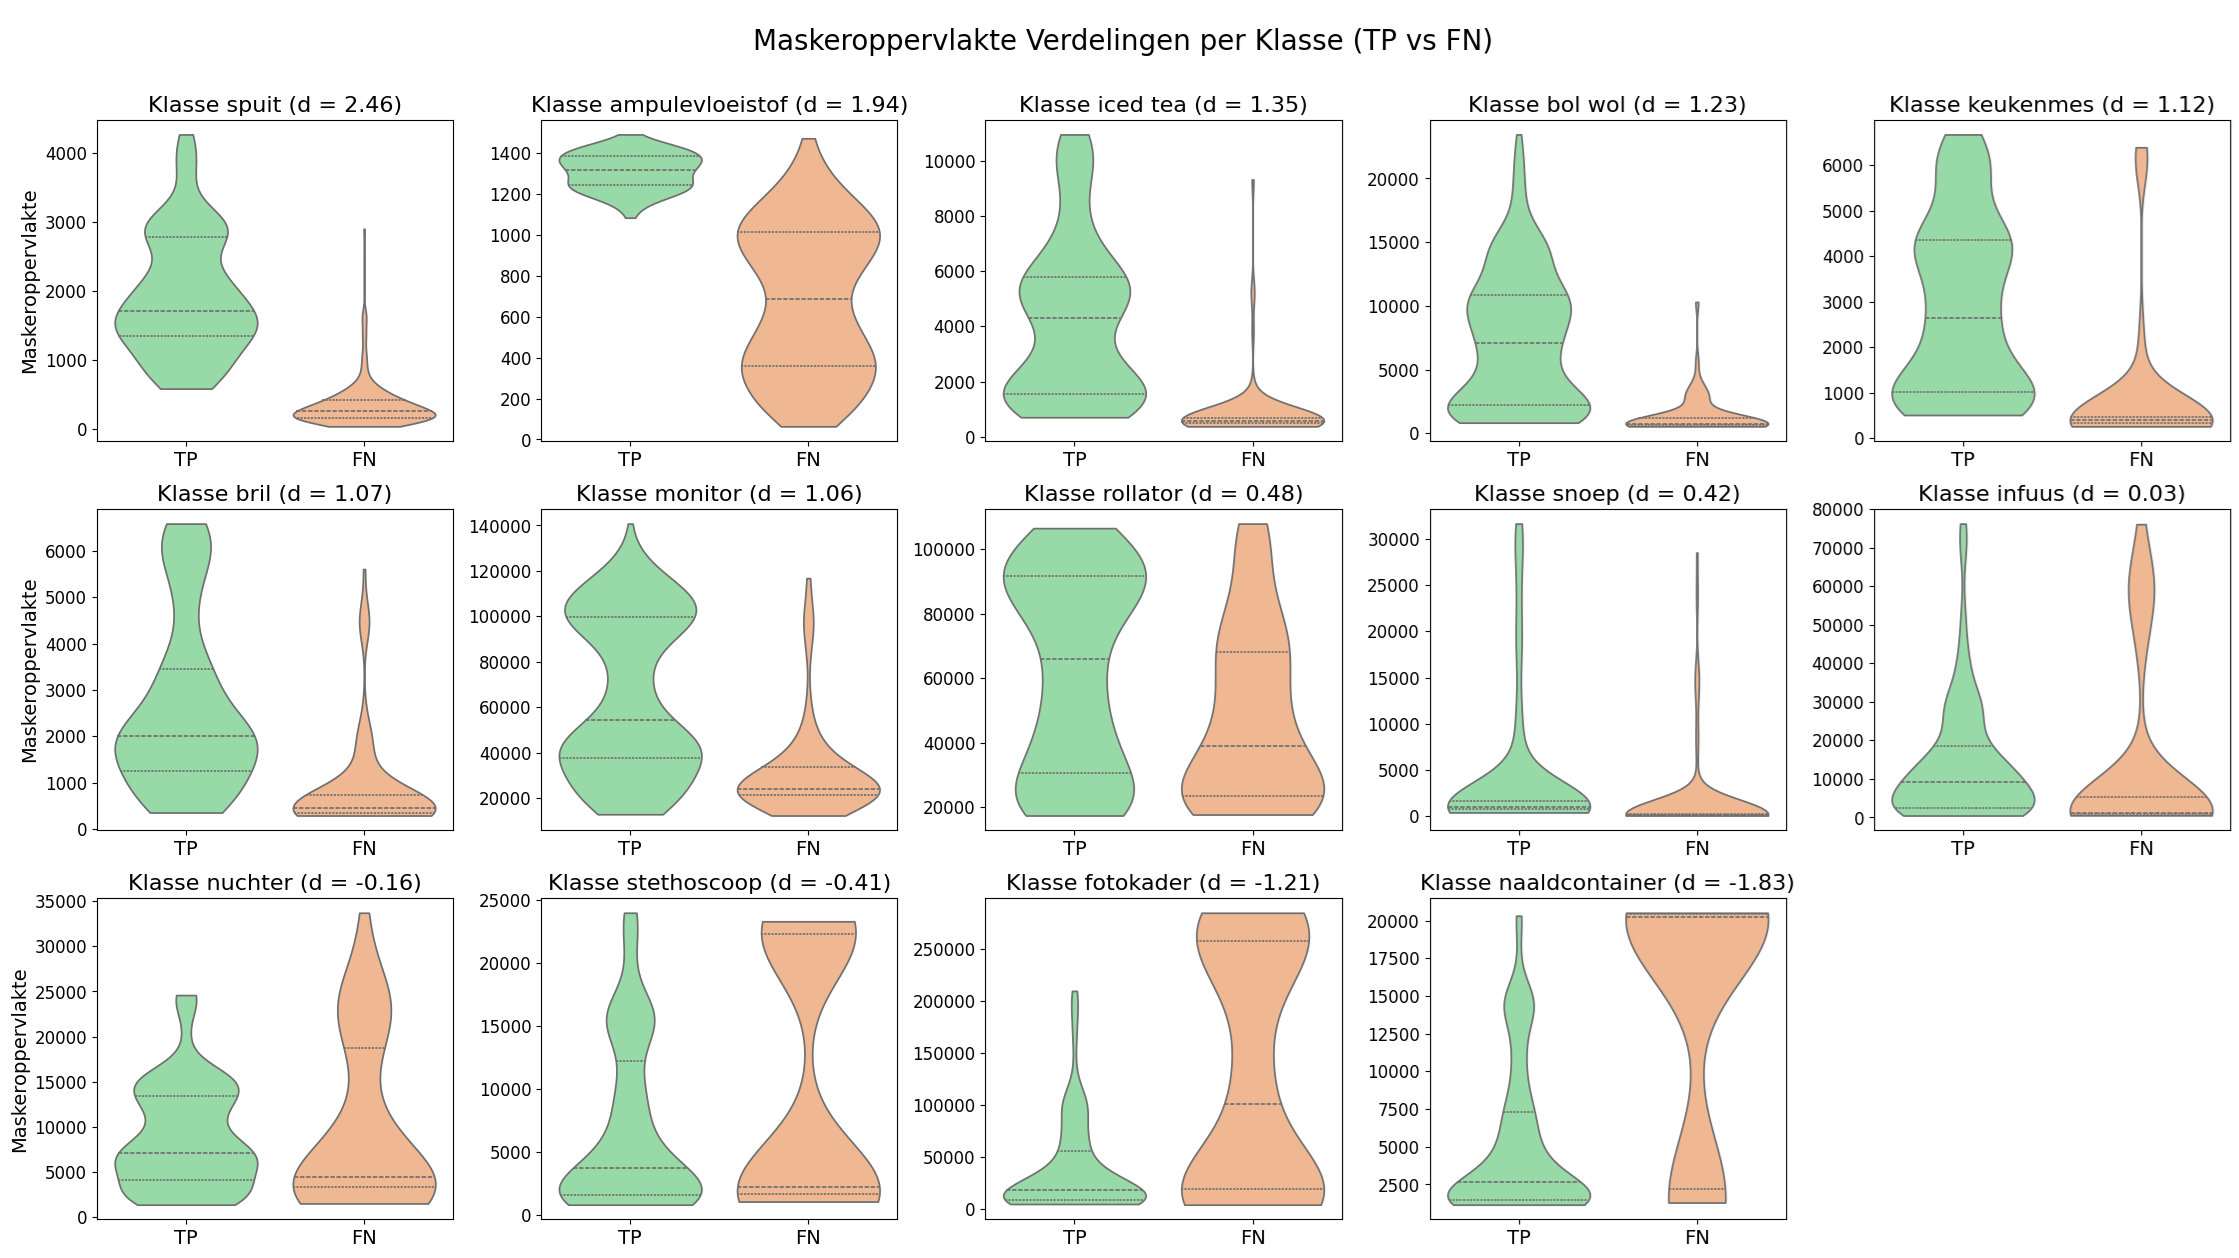
\includegraphics[width=1\textwidth]{mask-area-violin-plots.png}
  \caption[]{\label{fig:violinplot-fn-tp}
    Vioolplotten van de maskergroottes voor de waar-positieven (TP) en vals-negatieven (FN) per klasse.
    De breedte van elke viool geeft de dichtheid van de waarden aan, terwijl de hoogte de verdeling van de maskergroottes weergeeft.
  }
\end{figure}

Als aanvullende analyse werd ook manueel gekeken naar de uitsnedes van de vals-negatieven per klasse (op basis van de bounding box van de grondwaarheid).
Met deze drie analyses werden de volgende inzichten verkregen voor elke klasse die een `hoge' effectgrootte vertoonde (`\text{Cohen's d}' > 1):
\begin{itemize}
    \item \textbf{spuit en ampule vloeistof}: Beide objecten vertonen een zeer hoge effectgrootte.
    Dit is logisch, aangezien deze objecten klein en sterk doorzichtig zijn met een witte achtergrond. 
    Binnen de vioolplots van beide klassen zien we dat er voor de FN's een duidelijke grens is waaronder de maskeroppervlakten vallen. 
    Voor de spuit is dit rond de 600 pixels, en voor de ampule vloeistof rond de 1200 pixels.
    \item \textbf{iced tea, bol wol, keukenmes, en bril}: In de vioolplot van deze klassen zien we dat de FN's duidelijk geconcentreerd zijn onder de 1000 pixels,
    terwijl de TP's een veel bredere spreiding hebben. 
\end{itemize}
Daarnaast zijn er ook enkele klassen die een lage effectgrootte vertonen (`\text{Cohen's d}' tussen -0.5 en 0.5):
\begin{itemize}
    \item \textbf{rollator}: De rollator vertoont hier geen systematisch probleem. De `\text{Cohen's d}' waarde is hier waarschijnlijk een toeval.
    Een beter inzicht in de vals-negatieven voor dit object vergt een manuele inspectie van de opname, in combinatie met een overlay van de FastSAM-segmentaties, het blikpunt en de grondwaarheid.
    \item \textbf{snoep}: De vioolplot toont dat het aantal vals-negatieven toeneemt naarmate de maskergrootte kleiner wordt. 
    Toch vertoont het snoepje een hoog aantal TP's met een maskergrootte rond de 1000 pixels, in tegenstelling tot de hierboven besproken klassen.
    Dit valt waarschijnlijk te verklaren door het feit dat dit object een hoog kleurcontrast heeft met de achtergrond (groen snoepje op een witte tafel).
    Het FastSAM model heeft het dan ook gemakkelijker om dit object te segmenteren, zelfs wanneer het klein is.
    \item \textbf{infuus, nuchter en stethoscoop}: Deze klassen vertonen geen systematisch probleem ten opzichte van de maskergrootte.
    Een beter inzicht in de vals-negatieven van deze objecten zal net zoals de rollator een manuele inspectie vereisen. 
\end{itemize}
Tenslotte vertonen de fotokader en de naaldcontainer een hoge negatieve effectgrootte (`\text{Cohen's d}' < -1).
Bij de fotokader valt dit te verklaren door het feit dat binnen één van de opnames, de student het object van heel dichtbij bekeek.
Dit zorgde ervoor dat het object niet meer binnen de crop van 640x640 viel, waardoor het objectdetectiemodel geen voorspelling kon maken.
De negatieve effectgrootte van de naaldcontainer is waarschijnlijk niet representatief, aangezien deze klasse slechts 5.9\% van de support heeft als vals-negatieven.

Een consistent resultaat is dat de meeste klaasen een dunne, lange staart vertonen in de vioolplots voor de FN's. 
Dit valt, net zoals bij de vals-positieven, te verklaren door het feit dat de segmentatiemaskers van de FastSAM-tracking niet altijd volledig overeenkomen met die van de grondwaarheid.
Soms is een segmentatiemasker echter opgeschoven of kleiner dan die van de grondwaarheid, waardoor het blikpunt van de student net niet meer binnen de segmentatie valt.
Dit fenomeen resulteert dus ongeacht de maskergrootte in vals-negatieven.

Met de analyses die in dit hoofdstuk werden uitgevoerd, worden de onderzoeksvragen in het volgende hoofdstuk beantwoord.
